%% For double-blind review submission, w/o CCS and ACM Reference (max submission space)
\documentclass[sigplan,10pt,review,anonymous]{acmart}\settopmatter{printfolios=true,printccs=false,printacmref=false}
%% For double-blind review submission, w/ CCS and ACM Reference
%\documentclass[sigplan,10pt,review,anonymous]{acmart}\settopmatter{printfolios=true}
%% For single-blind review submission, w/o CCS and ACM Reference (max submission space)
%\documentclass[sigplan,10pt,review]{acmart}\settopmatter{printfolios=true,printccs=false,printacmref=false}
%% For single-blind review submission, w/ CCS and ACM Reference
%\documentclass[sigplan,10pt,review]{acmart}\settopmatter{printfolios=true}
%% For final camera-ready submission, w/ required CCS and ACM Reference
%\documentclass[sigplan,10pt]{acmart}\settopmatter{}

%% Use this to kill the ACM conference paragraph text from the first page for
%% review submissions (along with printacmref=false in documentclass)
\renewcommand\footnotetextcopyrightpermission[1]{} % removes footnote with conference information in first column
% \pagestyle{plain} % removes running headers (version 1)

% Remove running headers (version 2)
\fancyhead{}

%% Some recommended packages
\usepackage{booktabs}
\usepackage{subcaption}
%\usepackage{natbib}
%\usepackage{epsfig}
%\usepackage[utf8x]{inputenc}
\usepackage{amsmath}
\usepackage{amssymb}
\usepackage{algorithm}
\usepackage{algorithmicx}
\usepackage[noend]{algpseudocode}
%\usepackage{enumitem}      % adjust spacing in enums
%\usepackage{subfig}
%\usepackage{caption}
%\usepackage[hyphen]{url}

%% Custom packages
\usepackage{minted}
\usepackage{multirow}
\usepackage{rotating}
\usepackage{wrapfig}
\usepackage{tabu}
\usepackage{adjustbox}
\usepackage{pgfplots}
\usepackage{balance}

% \makeatletter
%     \def\balanceissued{unbalanced}%flag to indicate if \balance has been used
%     \let\oldbibitem\bibitem
%     \def\bibitem{%
%         \ifnum\thepage=\theTotPages%
%             \expandafter\ifx\expandafter\relax\balanceissued\relax\else%
%                 \balance%
%                 \gdef\balanceissued{\relax}\fi%
%             \else\fi%
%         \oldbibitem}
% \makeatother

%% Ignore acmart.cls loading natbib and let's use biblatex!
%% See: https://goo.gl/oocXmB
% \let\bibhang\relax
% \let\citename\relax
% \let\bibfont\relax
% \let\citeauthor\relax
% \let\Citeauthor\relax
% \let\citefullauthor\relax
% \let\citetext\relax
% \let\defcitealias\relax
% \let\citet\relax
% \let\citep\relax
% \let\Citep\relax
% \let\Citealt\relax
% \let\citealt\relax
% \let\citealp\relax
% \let\Citealp\relax
% \let\Citet\relax

% \expandafter\let\csname ver@natbib.sty\endcsname\relax

% \usepackage[natbib=true,backend=bibtex,firstinits=true,style=numeric-comp,sorting=nyt,defernumbers,maxnames=99,maxcitenames=99]{biblatex}

% \addbibresource{refs.bib}

%% OR: continue to use natbib (must be done for ACM pubs, apparently?!)

%% Custom colors that are colorblind safe, print friendly, and photocopy safe
\definecolor{purpleDark}{RGB}{94, 60, 153}
\definecolor{purpleLight}{RGB}{178, 171, 210}
\definecolor{orangeDark}{RGB}{230, 97, 1}
\definecolor{orangeLight}{RGB}{253, 184, 99}

%% Other custom colors
\definecolor{gray}{gray}{0.75}

%% Shortcuts
\newcommand{\ie}{\textit{i.e., }}
\newcommand{\eg}{\textit{e.g., }}
\newcommand{\CC}{C\nolinebreak\hspace{-.05em}\raisebox{.5ex}{\tiny\bf +}\nolinebreak\hspace{-.10em}\raisebox{.5ex}{\tiny\bf +}}

%% Units
\newcommand{\us}{\,$\mu$s}
\newcommand{\ms}{\,ms}
\newcommand{\KB}{\,KB}
\newcommand{\MB}{\,MB}
\newcommand{\GB}{\,GB}
\newcommand{\MHz}{\,MHz}
\newcommand{\GHz}{\,GHz}

%% Project name
\newcommand{\SYSTEM}{SwitchBox}
\newcommand{\SYSTEMURI}{https://git.xunn.io/closed-source/research/strongbox2}

%% Reference parts of the paper
\newcommand{\figref}[1]{Fig.~\ref{fig:#1}}
\newcommand{\figsref}[2]{Figures~\ref{fig:#1} and~\ref{fig:#2}}
\newcommand{\figrref}[2]{Figures~\ref{fig:#1}--\ref{fig:#2}}
\newcommand{\secref}[1]{Section~\ref{sec:#1}}
\newcommand{\secsref}[2]{Sections~\ref{sec:#1} and~\ref{sec:#2}}
\newcommand{\eqnref}[1]{Eqn.~\ref{eqn:#1}}
\newcommand{\eqnsref}[2]{Equations~\ref{eqn:#1} and~\ref{eqn:#2}}
\newcommand{\eqnrref}[2]{Equations~\ref{eqn:#1}--\ref{eqn:#2}}
\newcommand{\insref}[1]{Instruction~\ref{ins:#1}}
\newcommand{\tblref}[1]{Table~\ref{tbl:#1}}
\newcommand{\appref}[1]{Appendix~\ref{app:#1}}
\newcommand{\algoref}[1]{Algorithm~\ref{algo:#1}}

%% Math
\newcommand{\argmin}{\arg\!\min}
\newcommand{\argmax}{\arg\!\max}
\newcommand{\minimize}{minimize}
\newcommand{\optimize}{optimize}
\newcommand{\ceil}[1]{\lceil #1 \rceil}
\newcommand{\floor}[1]{\lfloor #1 \rfloor}
\newcommand{\st}{s.t.}

%% Custom
\newcommand{\PUNT}[1]{}
\newcommand{\TODO}[1]{\textcolor{gray}{\textbf{\ [TODO:\ #1]\ }}}
\newcommand{\FIX}[1]{\textcolor{red}{\textbf{\ [FIX:\ #1]\ }}}
\newcommand{\SystemURI}{(will be included in final paper)}%https://git.xunn.io/research/buselfs-public}

%% For algorithms
\newcommand{\LineComment}[1]{\Statex \hfill\textit{#1}}

%% Configurations

\DeclareCaptionFormat{subfig}{\figurename~#1#2#3}
\DeclareCaptionSubType*{figure}
\captionsetup[subfigure]{format=subfig,labelsep=colon,labelformat=simple}

% Options for pgfplots
\pgfplotsset{compat=1.8,compat/show suggested version=false}
\usetikzlibrary{plotmarks}
\usetikzlibrary{calc}
\pgfplotsset{
    /pgfplots/bar  cycle  list/.style={/pgfplots/cycle  list={%
        {black,fill=black!30!white,mark=none},%
        {black,fill=red!30!white,mark=none},%
        {black,fill=green!30!white,mark=none},%
        {black,fill=yellow!30!white,mark=none},%
        {black,fill=brown!30!white,mark=none},%
    }},
}

% Begin of externalization
\usetikzlibrary{external}
\tikzexternalize[prefix=out/]
\tikzexternalize

% Ensure letter paper
\pdfpagewidth=8.5in
\pdfpageheight=11in

% Further configure pgfplots and tikz
\usetikzlibrary{patterns}
\usepgfplotslibrary{groupplots}
\pgfplotsset{
    every axis label/.append style={font=\small},
    tick label style={font=\small},
}

\pdfstringdefDisableCommands{
    \def\\{}
    \def\unskip{}
    \def\texttt#1{<#1>}
}

\graphicspath{{./figs/}{./charts/}}

\pgfkeys{
    /pgf/number format/precision=1,
    /pgf/number format/fixed zerofill=true,
}

\pgfplotsset{
    nodes near coords greater equal only/.style={
        small value/.style={
            /tikz/coordinate,
        },
        every node near coord/.append style={
            check for small values/.code={
                \begingroup
                \pgfkeys{/pgf/fpu}
                \pgfmathparse{\pgfplotspointmeta<#1}
                \global\let\result=\pgfmathresult
                \endgroup
                \pgfmathfloatcreate{1}{1.0}{0}
                \let\ONE=\pgfmathresult
                \ifx\result\ONE
                    \pgfkeysalso{/pgfplots/small value}
                \fi
            },
            check for small values
        },
    },
}

%% Conference information
%% Supplied to authors by publisher for camera-ready submission;
%% use defaults for review submission.
\acmYear{2019}
\acmConference[ASPLOS'19]{}{}{}
\acmBooktitle{}
\acmPrice{}
\acmDOI{} % \acmDOI{10.1145/nnnnnnn.nnnnnnn}
\acmISBN{} % \acmISBN{978-x-xxxx-xxxx-x/YY/MM}
\startPage{1}

%% Copyright information
%% Supplied to authors (based on authors' rights management selection;
%% see authors.acm.org) by publisher for camera-ready submission;
%% use 'none' for review submission.
%\setcopyright{none}
\setcopyright{acmcopyright}
%\setcopyright{acmlicensed}
%\setcopyright{rightsretained}
\copyrightyear{2019}           %% If different from \acmYear

%% Citation style
%\citestyle{acmauthoryear}  %% For author/year citations
\citestyle{acmnumeric}      %% For numeric citations
%\setcitestyle{nosort}      %% With 'acmnumeric', to disable automatic
                            %% sorting of references within a single citation;
                            %% e.g., \cite{Smith99,Carpenter05,Baker12}
                            %% rendered as [14,5,2] rather than [2,5,14].
%\setcitestyle{nocompress}   %% With 'acmnumeric', to disable automatic
                            %% compression of sequential references within a
                            %% single citation;
                            %% e.g., \cite{Baker12,Baker14,Baker16}
                            %% rendered as [2,3,4] rather than [2-4].


%%%%%%%%%%%%%%%%%%%%%%%%%%%%%%%%%%%%%%%%%%%%%%%%%%%%%%%%%%%%%%%%%%%%%%
%% Note: Authors migrating a paper from traditional SIGPLAN
%% proceedings format to PACMPL format must update the
%% '\documentclass' and topmatter commands above; see
%% 'acmart-pacmpl-template.tex'.
%%%%%%%%%%%%%%%%%%%%%%%%%%%%%%%%%%%%%%%%%%%%%%%%%%%%%%%%%%%%%%%%%%%%%%


\begin{document}

%% Title information
%\title[StrongBox: Confidentiality, Integrity, and Performance]{StrongBox:
%Confidentiality, Integrity, and Performance using Stream Ciphers for Full Drive
%Encryption}
\title{SwitchBox: Security, Energy, and Performance Tradeoffs Leveraging LFS
Behavior in Stream Cipher Based Full Drive Encryption}
%% [Short Title] is optional;
                                        %% when present, will be used in
                                        %% header instead of Full Title.
%\titlenote{with title note}            %% \titlenote is optional;
                                        %% can be repeated if necessary;
                                        %% contents suppressed with 'anonymous'
%\subtitle{Subtitle}                    %% \subtitle is optional
%\subtitlenote{with subtitle note}      %% \subtitlenote is optional;
                                        %% can be repeated if necessary;
                                        %% contents suppressed with 'anonymous'


%% Author information
%% Contents and number of authors suppressed with 'anonymous'.
%% Each author should be introduced by \author, followed by
%% \authornote (optional), \orcid (optional), \affiliation, and
%% \email.
%% An author may have multiple affiliations and/or emails; repeat the
%% appropriate command.
%% Many elements are not rendered, but should be provided for metadata
%% extraction tools.

%% Authors with single affiliation
%% \email is recommended
\author{Bernard Dickens III}
\affiliation{
  %\position{Position1}
  %\department{Department1}              %% \department is recommended
  \institution{University of Chicago}
  % \streetaddress{5801 S Ellis Ave}
  % \city{Chicago}
  % \state{IL}
  % \postcode{60637}
  % \country{USA}
}
\email{bd3@cs.uchicago.edu}

\author{Haryadi S. Gunawi}
\affiliation{
  %\position{Position1}
  %\department{Department1}              %% \department is recommended
  \institution{University of Chicago}
  % \streetaddress{5801 S Ellis Ave}
  % \city{Chicago}
  % \state{IL}
  % \postcode{60637}
  % \country{USA}
}
\email{haryadi@cs.uchicago.edu}

\author{David Cash}
\affiliation{
  %\position{Position1}
  %\department{Department1}              %% \department is recommended
  \institution{University of Chicago}
  % \streetaddress{5801 S Ellis Ave}
  % \city{Chicago}
  % \state{IL}
  % \postcode{60637}
  % \country{USA}
}
\email{davidcash@cs.uchicago.edu}


\author{Henry Hoffmann}
\affiliation{
  %\position{Position1}
  %\department{Department1}              %% \department is recommended
  \institution{University of Chicago}
  % \streetaddress{5801 S Ellis Ave}
  % \city{Chicago}
  % \state{IL}
  % \postcode{60637}
  % \country{USA}
}
\email{hankhoffmann@cs.uchicago.edu}


%% Abstract
%% Note: \begin{abstract}...\end{abstract} environment must come
%% before \maketitle command
\begin{abstract}

Recent work on Full Drive Encryption shows that stream ciphers achieve
significantly improved performance over block ciphers while offering stronger
security guarantees. However, optimizing for performance often conflicts with
other key concerns like energy usage and desired security properties. In this
paper we present SwitchCrypt, a software mechanism that navigates the tradeoff
space made by balancing competing security and latency requirements via
\emph{cipher switching} in space or time. Our key insight in achieving
low-overhead switching is to leverage the overwrite-averse, append-mostly
behavior of underlying solid-state storage to trade throughput for reduced
energy use and/or certain security properties. We implement SwitchCrypt on an
ARM big.LITTLE mobile processor and test its performance under the popular F2FS
file system. We provide empirical results demonstrating the conditions under
which different switching strategies are optimal through the exploration of four
cases studies. In one study, where we require the filesystem to react to a
shrinking energy budget by switching ciphers, we find that SwitchCrypt achieves
up to a 3.3x total energy use reduction compared to a static approach using only
the Freestyle stream cipher. In another case, where we allow the user to
manually switch between ChaCha20 and Freestyle stream ciphers dynamically, we
achieve a 1.6x to 4.8x reduction in I/O latency compared to prior static
approaches.

\end{abstract}



%% 2012 ACM Computing Classification System (CSS) concepts
%% Generate at 'http://dl.acm.org/ccs/ccs.cfm'.
% \begin{CCSXML}
% \end{CCSXML}

\ccsdesc[500]{Information systems~Data encryption}
\ccsdesc[300]{Information systems~Flash memory}
\ccsdesc[500]{Security and privacy~Block and stream ciphers}
\ccsdesc[500]{Security and privacy~Hash functions and message authentication codes}
\ccsdesc[300]{Security and privacy~Key management}
\ccsdesc[100]{Security and privacy~Tamper-proof and tamper-resistant designs}
\ccsdesc[500]{Software and its engineering~File systems management}
%% End of generated code


%% Keywords
%% comma (ASPLOS uses SEMICOLONS!) separated list
\keywords{}
%% \keywords are mandatory in final camera-ready submission


%% \maketitle
%% Note: \maketitle command must come after title commands, author
%% commands, abstract environment, Computing Classification System
%% environment and commands, and keywords command.
\maketitle
%\renewcommand{\shortauthors}{Dickens et al.} %% If there are a lot of authors...

%% It begins:
\section{Introduction}\label{sec:introduction}

There are several important concerns modern filesystems must balance. Paramount
among them are: security of data at rest; performance, \ie{I/O latency or
throughput}; and overall energy budget. However, these concerns exist in
contention with one another.

The state of the art for securing data at rest is Full-Drive Encryption
(FDE)\footnote{The common term is full-\emph{disk} encryption, but this work
targets SSDs, so we use \emph{drive}.}. FDE employs a \emph{cryptographic
cipher} to encrypt, decrypt, and authenticate backing store contents on the fly.
Understandably, this process impacts system performance and energy use
considerably. Yet, end users expect their device to be secure \emph{and}
performant \emph{and} energy efficient. The obvious solution is to balance these
concerns with respect to the most general use case, but this is not always
desirable. \TODO{Introduce two examples: 1) Android M FDE example from
Google~\cite{AndroidM}. 2) Another example from someone
else~\cite{AnotherExample}.}

FDE's impact on performance and energy efficiency depends on choice of
filesystem/mapper and the choice of cipher, as different ciphers express
different performance and efficiency characteristics while offering contrasting
security guarantees. In this way, cipher choice is perhaps the most important.

The standard choice for FDE is the relatively slow AES~\cite{AES} \emph{block
cipher} in XTS mode (AES-XTS)~\cite{AES-XTS}. Prior work~\cite{StrongBox}
introduced the motivation and method for using \emph{stream ciphers} like the
high performance ChaCha20~\cite{ChaCha20} cipher for FDE in lieu of AES-XTS.
More recent work achieves something similar, such as Google's HBSH~\cite{HBSH}
(hash, block cipher, stream cipher, hash), Adiantum~\cite{Adiantum}, and others.

The benefits of choosing a more performant cipher include increased filesystem
performance(\ie{overall reduced FDE overhead}), reduced energy use, and the
ability to encrypt devices that would otherwise be too slow or
energy-inefficient to support FDE, as was the case with many mid- and low-tier
Android devices at the time FDE was considered for Android M.

And ChaCha20 is not the only stream cipher we can choose for FDE. Other stream
ciphers exist with a variety of different performance characteristics and
opposing security properties. Some of these include: ChaCha variants with
different round counts (e.g., ChaCha8 \cite{ChaCha8} and ChaCha20
\cite{ChaCha20}) or special modes (e.g., Freestyle~\cite{Freestyle}),
SalsaX~\cite{SalsaX}, AES in counter mode (AES-CTR)~\cite{AES-CTR},
Rabbit~\cite{Rabbit}, Sosemanuk~\cite{Sosemanuk},, et cetera.

In this way, the choice of (stream) cipher can be viewed as a key
\emph{configuration} parameter for systems supporting FDE; \ie{the configuration
providing the fastest I/O throughput is almost always different than the
configuration providing the strongest security guarantees, and both may differ
from the configuration that uses the least amount of energy}. Further, while the
cipher choice can be configured statically at compile- or boot-time given some
generic case, in traditional FDE, these configurations cannot adapt to changes
that might arise while the system is running. Examples include changes in
resource availability, runtime environment, energy-budget and OS ``battery
saver'' functionality.

Hence, any static configuration will inevitably sacrifice one concern for
another, even when it is not optimal. But what if our system did not have to sit
at a static configuration point, even when another configuration became more
optimal later on?

\subsection{Our Contributions}

We introduce a simple scheme to quantify the security ``strength'' of
arbitrary stream ciphers based on a subset of properties relevant to
FDE.

Using this scheme, we then define a novel tradeoff space of competing concerns:
total energy use, our notion of cipher strength, and the performance
characteristics of various stream ciphers in the context of FDE.

Finally, we present SwitchBox, a novel design substantively expanding on prior
work by 1) decoupling the cipher implementation from the encryption mechanism,
2) allowing ciphertext from different ciphers to coexist side-by-side on the
same drive as independent units, 3) employing various \emph{switching
strategies} to ``re-cipher'' those independent units dynamically at run-time.
SwitchBox accomplishes these without significant overhead, allowing us to
navigate our space of cipher configurations online, always ensuring that the
system is sitting at the most optimal configuration.

\TODO{We demonstrate SwitchBox's effectiveness on ...; we measure using ...; we
further demonstrate with use cases ...}

\TODO{Short explanation of the remaining structure of the paper.}

\section{Motivation}\label{sec:motivation}

\subsection{Example: Filesystem Reacts to ``Battery Saver''}

\PUNT{\begin{figure}[ht] \textbf{Linearity Between Baseline Cipher Latency and
Energy Use}\par\medskip
   \centering
   {\begin{tikzpicture}[baseline]

    \pgfmathsetmacro{\ymax}{1} % set the maximum y value
    \pgfmathsetmacro{\ymaxbreak}{1.1} % set the y value at which overflow is drawn

    \begin{axis}[
        %axis x line*=bottom,
        only marks,
        height=6cm,
        width=\linewidth,
        tick align=outside,
        tick pos=bottom, % make sure ticks only appear at the bottom and left axes
        tick style={ black },
        y tick label style={ /pgf/number format/fixed, /pgf/number format/precision=0 },
        grid style={ dotted, gray },
        %every node near coord/.append style={font=\tiny},
        %
        % magic to make the numbers appear above the overly long bars:
        % visualization depends on={rawy \as \rawy}, % save original y values
        % restrict y to domain*={ % now clip/restrict any y value to ymax
        %     \pgfkeysvalueof{/pgfplots/ymin}:\ymaxbreak
        % },
        % after end axis/.code={ % draw squiggly line indicating break
        %     \draw [semithick, white, decoration={snake,amplitude=0.1mm,segment length=0.75mm,post length=0.375mm}, decorate] (rel axis cs:0,1.01) -- (rel axis cs:1,1.01);
        % },
        % nodes near coords={\color{.!75!black}\pgfmathprintnumber\rawy}, % print the original y values (darkened in case they are too light)...
        % nodes near coords greater equal only=\ymax, % ... but ONLY if they are >= ymax
        % clip=false, % allow clip to protrude beyond ymax
        % Custom stuff to edit per template
        %
        xlabel={\footnotesize Energy (normalized)},
        xlabel near ticks,
        xmin=0, xmax=1,
        xtick={ 0, 1 },
        %enlarge x limits=0.2, % add some breathing room along the x axis's sides
        %major x tick style=transparent,
        %
        ylabel={\footnotesize Latency (normalized)},
        ylabel near ticks,
        ylabel shift={-1mm},
        ymajorgrids=true,
        ymin=0, ymax=\ymax,
        ytick={ 0, 1 },
        restrict x to domain=0:1,
        %yticklabels={ 0, 0.5, 1.5, 2 },
        % extra y ticks={1},
        % extra y tick style={grid=major, grid style={dashed, black}},
        % extra y tick label={\empty},
        %bar width=4.5pt, % change size of bars
        %
        legend cell align=left,
        legend style={ column sep=1ex },
        legend style={
            draw=none,
            legend columns=2,
            at={(0.5,1.02)},
            anchor=south,
        },
    ]
        \addplot [blue] table [
            only marks,
            x=energy,
            y=latency,
            discard if symbol not={iop}{4k-r},
            discard if symbol not={order}{seq},
            col sep=space,
        ] {charts/tradeoff-baseline.dat};
        \addlegendentry{\scriptsize 4K I/O}
        \addplot [] table [
            only marks,
            x=energy,
            y=latency,
            discard if symbol not={iop}{512k-r},
            discard if symbol not={order}{seq},
            col sep=space
            ] {charts/tradeoff-baseline.dat};
        \addlegendentry{\scriptsize 512K/5M/40M I/O}
        \addlegendimage{mark=none, red, thick}
        \addlegendentry{\scriptsize Regression}
        \addplot [] table [
            only marks,
            x=energy,
            y=latency,
            discard if symbol not={iop}{5m-r},
            discard if symbol not={order}{seq},
            col sep=space
        ] {charts/tradeoff-baseline.dat};
        \addplot [] table [
            only marks,
            x=energy,
            y=latency,
            discard if symbol not={iop}{40m-r},
            discard if symbol not={order}{seq},
            col sep=space
        ] {charts/tradeoff-baseline.dat};
        \addplot [blue] table [
            only marks,
            x=energy,
            y=latency,
            discard if symbol not={iop}{4k-w},
            discard if symbol not={order}{rnd},
            col sep=space,
        ] {charts/tradeoff-baseline.dat};
        \addplot [] table [
            only marks,
            x=energy,
            y=latency,
            discard if symbol not={iop}{512k-w},
            discard if symbol not={order}{rnd},
            col sep=space
        ] {charts/tradeoff-baseline.dat};
        \addplot [] table [
            only marks,
            x=energy,
            y=latency,
            discard if symbol not={iop}{5m-w},
            discard if symbol not={order}{rnd},
            col sep=space
        ] {charts/tradeoff-baseline.dat};
        \addplot [] table [
            only marks,
            x=energy,
            y=latency,
            discard if symbol not={iop}{40m-w},
            discard if symbol not={order}{rnd},
            col sep=space
        ] {charts/tradeoff-baseline.dat};
        \addplot [sharp plot, mark=none, red] table [
            x=energy,
            y={create col/linear regression={y=latency}},
            col sep=space
        ] {charts/tradeoff-baseline.dat};
    \end{axis}%
\end{tikzpicture}%
} \caption{Comparison of cipher
   configuration median sequential and random latency versus median total energy
   use per I/O operation size (4KB, 512KB, 5MB, 40MB) without switching. The
   relationship between latency and total energy use is linear for the cipher
   configurations we examine in this paper.}
  \label{fig:linearity-latency-energy}
\end{figure}}

Suppose we have an ARM-based ultra-low-voltage netbook provided to us by our
employer. As this is an enterprise device, our employer requires that 1) our
drive is fully encrypted at all times and 2) our encrypted data is constantly
backed up to an offsite system. The industry standard in full drive encryption
is AES-XTS, so we initialize our drive with it. Given these requirements, three
primary concerns present themselves.

First, it is well known that FDE using AES-XTS adds significant latency and
power overhead to I/O operations, especially on mobile and battery-constrained
devices~\cite{google-engadget, android-M-mobile-motivation,
android-M-mobile-motivation-2}. To keep our drive encrypted at all times with
AES-XTS means we must accept this hit to performance and battery life. Worse, if
our device does not support hardware accelerated AES, performance can be
degraded even further; I/O latency can be as high as 3-5x~\cite{StrongBox}.
Hardware accelerated AES is hardly ubiquitous, and the existence of myriad
devices that do not support it cannot simply be ignored, hence Google's
investment in Adiantum~\cite{Adiantum}.

Second, AES-XTS was designed to mitigate threats to drive data ``at rest,''
which implies an attacker cannot access snapshots of our encrypted data nor
manipulate that data without it being immediately obvious to us. With access to
multiple snapshots of a drive's AES-XTS-encrypted contents, an attacker can
passively glean information about the plaintext over time, possibly violating
data confidentiality~\cite{XEX, XTS}. Similarly, an attacker that can flip
encrypted bits without drawing our attention will corrupt any eventual
plaintext. Unfortunately, in real life, data rarely remains ``at rest'' in this
way. In our example, our employer requires we back up the contents of our drive
to some offsite backup service. This service will receive periodic snapshots of
the encrypted state of our drive, violating our invariant.

Third, our system is battery constrained, placing a cap on our energy budget
that can change at any moment.

To alleviate the performance concern, we can choose a stream cipher like
ChaCha20 rather than the AES-XTS block cipher. Using StrongBox, an encryption
driver built for ChaCha20-based FDE, we can achieve on average a 1.7x speedup
and a commensurate reduction in energy use~\cite{StrongBox}.

When it comes to the security concern, StrongBox solves both the snapshot and
integrity problems by 1) never writing data encrypted with the same key to the
same location and 2) tracking drive state using a Merkle tree and monotonic
counter supported by trusted hardware to prevent rollbacks. This ensures data
manipulations cannot occur and guarantees confidentiality even when snapshots
are compared. Unfortunately, restoring from a backup necessitates a forced
rollback of drive state, potentially opening us back up to
confidentiality-violating snapshot comparison attacks~\cite{StrongBox}.

To truly address the security concern requires a cipher with an additional
security property: ciphertext randomization. Using Freestyle~\cite{Freestyle}, a
ChaCha20-based stream cipher that supports ciphertext randomization, we can
guarantee data confidentiality even after a rollback of drive state occurs. So,
we switch to an encryption driver that supports Freestyle.

Unfortunately, like AES-XTS, Freestyle has significant overhead compared to the
original ChaCha20. In exchange for stronger security properties, Freestyle is up
to 1.6x slower than ChaCha20, uses more energy, has a higher initialization
cost, and expands the ciphertext which reduces total writeable drive
space~\cite{Freestyle}.

Further complicating matters is our final concern: a constrained energy budget.
Our example system is battery constrained. Even if we accepted trading off
performance, drive space, and energy for security in some situations, in other
situations we might prioritize reducing total energy use. For example, when we
trigger ``battery saver'' mode, we expect our device to conserve as much energy
as possible. It would be ideal if our device could pause backups and the
encryption driver could switch from the ciphertext randomizing Freestyle
configuration back to our high performance energy-efficient ChaCha20
configuration when conserving energy is a top priority, and then switch back to
the Freestyle configuration when we connect to a charger and backups are
eventually resumed.

With SwitchCrypt, we can dynamically trade off between these two configurations
and others without compromising security or performance or requiring the device
be restarted.

\subsection{Key Challenges}

To trade off between different cipher configurations, we must address three key
challenges. First, we must determine what cipher configurations are most
desirable in which contexts and why. This requires we \emph{quantify} the
desirable properties of these configurations. Second, we must have some way to
encrypt independent storage units with any one of these configurations. This
requires we \emph{decouple} cipher implementations from the encryption process
used in prior work. Third, we need to determine when to re-encrypt those units,
which configuration to use, and where to store the output, all with minimal
overhead. This requires we implement efficient cipher \emph{switching
strategies}.

\textbf{Quantifying the properties traded off between configurations.} To obtain
a space of configurations that we might reason about, it is necessary to compare
certain properties of stream ciphers useful in the FDE context. However,
different ciphers have a wide range of security properties, performance
profiles, and output characteristics, including those that randomize their
outputs and those with non-length-preserving outputs---\ie{the cipher outputs
more data than it takes in}. To address this, we propose a framework for
quantitative cipher comparison in the FDE context; we use this framework to
define our configurations.

\textbf{Decoupling ciphers from the encryption process.} To flexibly switch
between configurations in SwitchCrypt requires a generic cipher interface. This
is challenging given the variety of inputs required by various stream ciphers,
the existence of non-length-preserving ciphers, and other differences. We
achieve the required generality by defining independent storage units called
\emph{nuggets}; we borrow this terminology from prior work (see
\cite{StrongBox}) to easily differentiate our logical blocks (nuggets) from
physical drive and other storage blocks. And since they are independent, we can
use our interface to select any configuration to encrypt or decrypt any nugget
at any point.

\textbf{Implementing efficient switching strategies.} Finally, to determine when
to switch a nugget's cipher and to where we commit the output, we implement a
series of high-level policies we call \textit{cipher switching strategies}.
These strategies leverage our generic cipher interface and flexible drive layout
to selectively ``re-cipher'' groups of nuggets, whereby the key and the cipher
used to encrypt/decrypt a nugget are switched at runtime. These strategies allow
SwitchCrypt to move from one configuration point to another or even settle on
optimal configurations wholly unachievable with prior work. The challenge
here is to accomplish this while minimizing overhead.

\section{SwitchCrypt Design} \label{sec:design}

What follows is a brief overview of SwitchCrypt's design
(\cref{subsec:overview}). We then discuss our novel, general API for
\emph{decoupling} the cipher implementations from the encryption/decryption
process (\cref{subsec:api}), describe and contrast three cipher \emph{switching
strategies} (\cref{subsec:strategies}), and then detail our scheme to
\emph{quantify} cipher strength (\cref{subsec:quantify}). Finally, we revisit
the battery saver example and summarize how the SwitchCrypt components fit
together (\cref{subsec:summary}). In this section, we first give a brief
overview of SwitchCrypt's design.

\subsection{SwitchCrypt Overview} \label{subsec:overview}

Like StrongBox, SwitchCrypt sits between a Log-structured File System (LFS) and
the backing storage, dividing it into a series independent same-size logical
units called \emph{nuggets}. A nugget consists of one or more contiguous
physical drive blocks with per-nugget metadata indicating which cipher was used
to encrypt the nugget.

SwitchCrypt uses the nugget layout to 1) track, detect, and handle overwrites,
2) limit the maximum length of any plaintext input to ciphers, thus amortizing
the overhead incurred during encryption~\cite{StrongBox}, and 3) independently
switch the cipher used to crypt individual nuggets.

\PUNT{\begin{figure}[t]
\centering
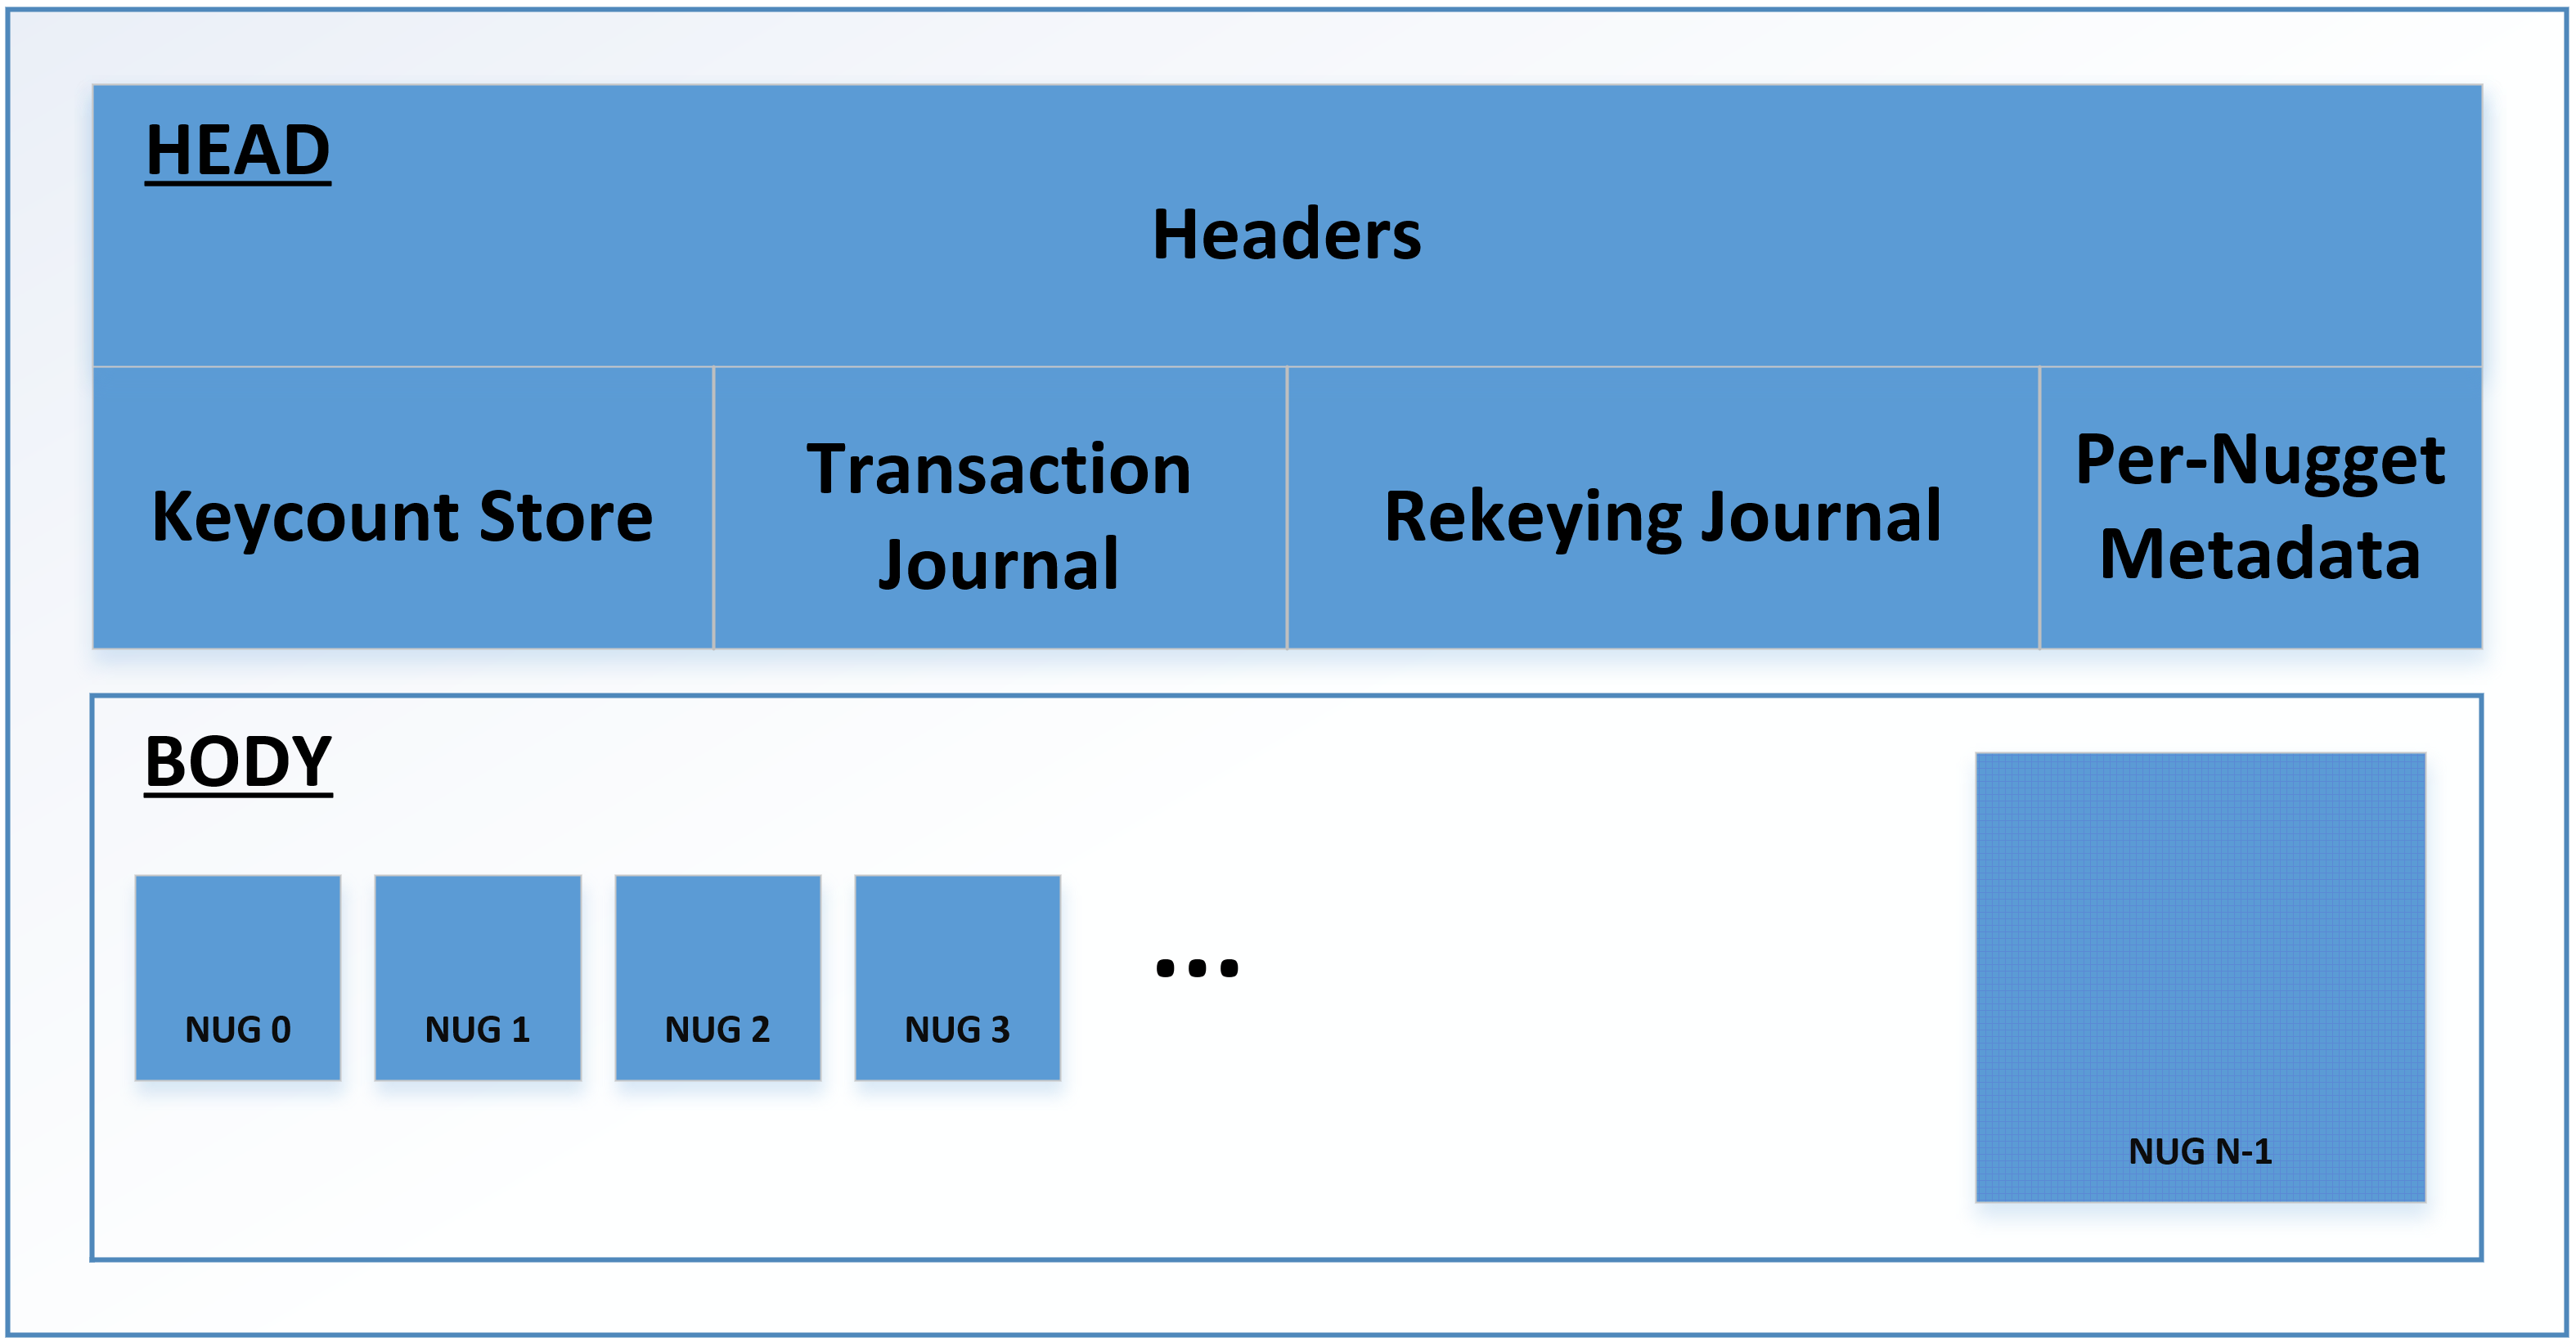
\includegraphics[width=\linewidth]{backstore.png}
 \caption{Layout of SwitchCrypt's backing storage.}\label{fig:backstore2}
\end{figure}}

\begin{figure}[ht]
   \centering
   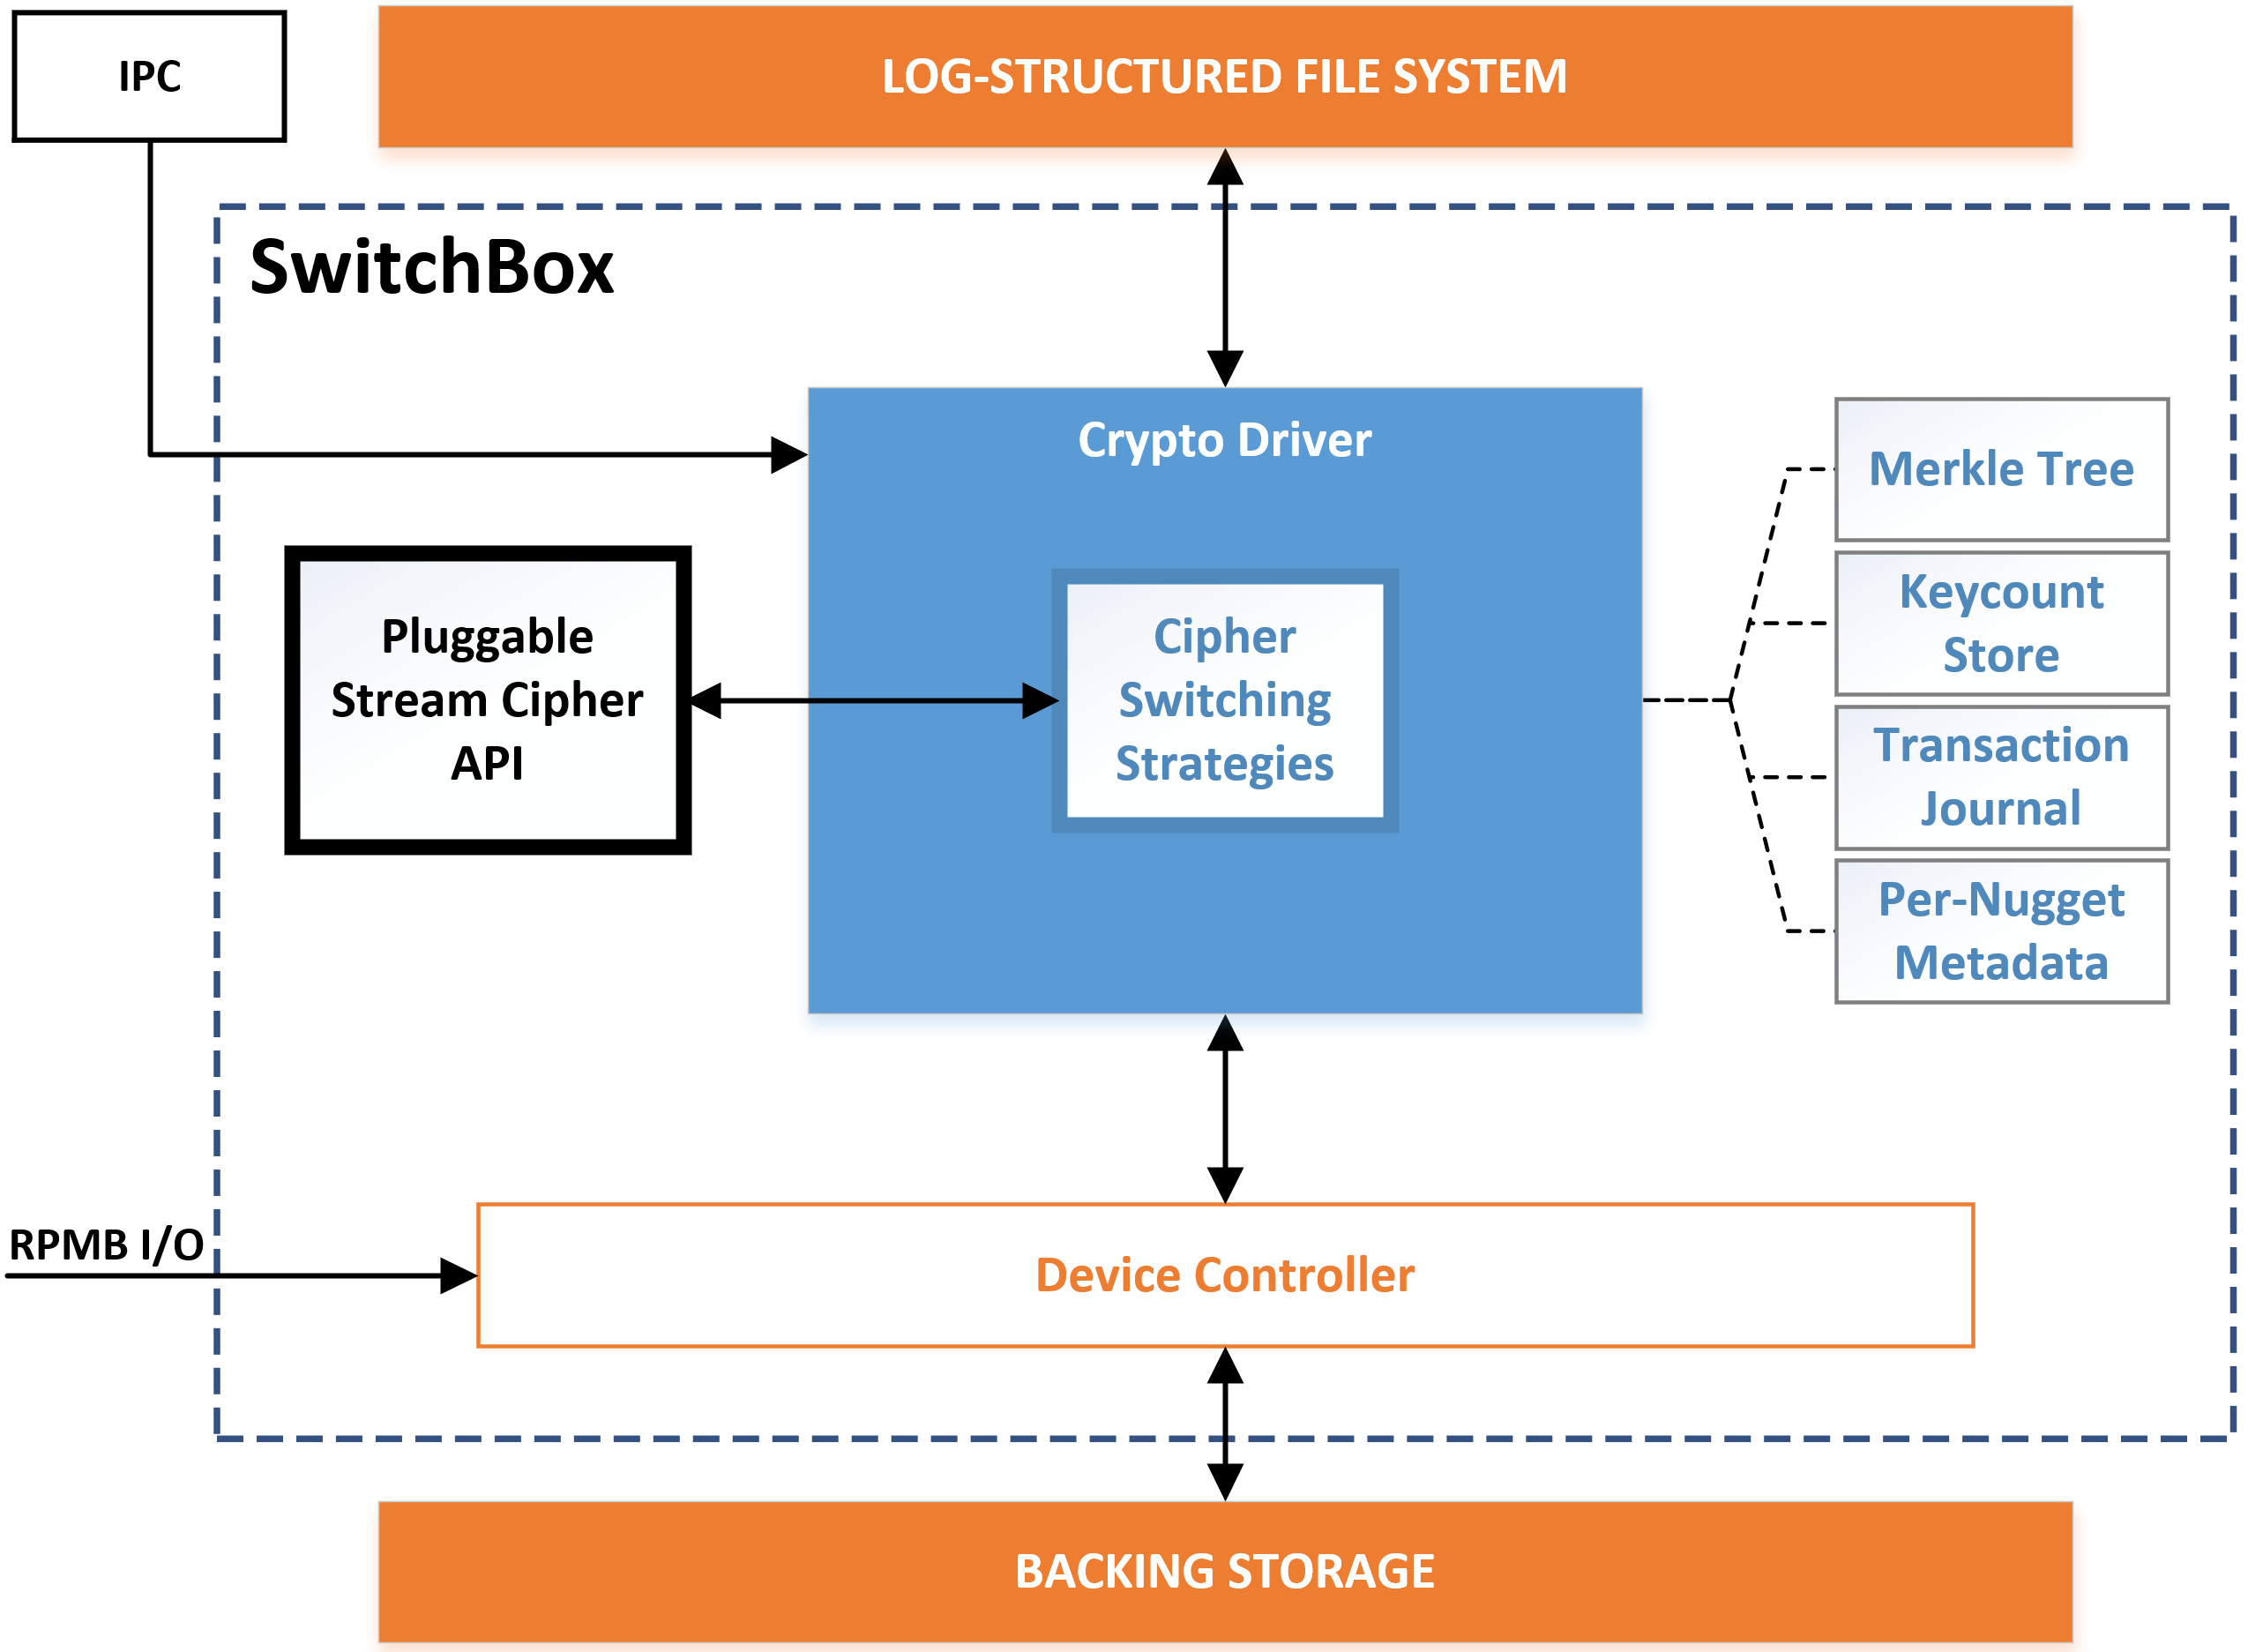
\includegraphics[width=\linewidth]{overview.png}
   \caption{Overview of the SwitchCrypt construction.}\label{fig:overview}
\end{figure}

\figref{overview} provides an overview of the SwitchCrypt design. SwitchCrypt is
composed of the cryptographic driver---responsible for executing our
\emph{switching strategies}---and six components. The first four components
belong to StrongBox: an in-memory \emph{merkle tree}; two drive-backed byte
arrays, \ie{the \emph{keycount store} and the \emph{transaction journal}}; a
globally persistent cryptographically secure monotonic counter~\cite{StrongBox}.
Our design adds the final two components: a flexible drive-backed store for
cipher-specific \emph{per-nugget metadata} and the \emph{generic stream cipher
API}.

The \emph{merkle tree} ensures the integrity of all data on a per-nugget level.
The \emph{keycount store} keeps track of each nugget's 64-bit cryptographic key.
The \emph{transaction journal} keeps track of writes to nuggets, allowing
SwitchCrypt to detect and respond to overwrites. The \emph{monotonic counter}
prevents the system state from being rolled back. The \emph{per-nugget metadata}
is a drive-backed array where extra cryptographic material is stored depending
on the cipher used to encrypt the nugget. The size of the array is determined by
ciphers loaded through the \emph{generic stream cipher API}.

\subsection{Generic Stream Cipher API} \label{subsec:api}

There are \emph{many} ciphers we might use with SwitchCrypt, each with various
input requirements and output considerations. A key difference with prior work
is that SwitchCrypt must be able to encrypt and decrypt arbitrary nuggets
without worrying about a cipher's implementation details; prior approaches could
have cipher-specific implementations because they did not consider switching.
Thus, the cipher-specific details must be handled with care or security is
violated. With our novel cipher API, we present an interface that
\emph{decouples} cipher implementations from the encryption/decryption process.
This allows any cipher to be integrated into SwitchCrypt without modification or
special considerations. Hence, different stream ciphers become interchangeable
when they would normally be incompatible, preventing us from trading them off
one another.

The API is accessible at three levels:

\begin{enumerate}
   \item \textbf{\texttt{crypt\_data}}\\\texttt{crypt\_data}
   operates at a fine-grain level independent of SwitchCrypt's internals.
   Implementations receive an index and offset and are expected to return some
   number of bytes, \ie{a keystream}, which is XORed with nugget contents. At
   this level, there is no distinction made between encryption and decryption
   since both are accomplished with a simple XOR. This API level has the lowest
   implementation overhead and least flexibility.

   \item \textbf{\texttt{crypt\_data\_low}}\\\texttt{crypt\_data\_low}
   is identical to \texttt{crypt\_data} but provides a slightly lower level of
   abstraction when accessing the backing store, giving implementations more
   control over the XORing process. This is useful for less flexible ciphers but
   comes at the cost of increased implementation overhead.

   \item \textbf{\texttt{read\_data}} and \textbf{\texttt{write\_data}}\\
   These operate at a coarse-grain level tightly integrated with SwitchCrypt
   internals. Implementations are expected to handle all stages of cipher
   switching manually. Unlike the other two levels, encryption and decryption
   are distinct concerns. \texttt{read\_data} handles decryption during reads.
   \texttt{write\_data} handles encryption during writes. In exchange for
   maximum flexibility, there is significant implementation overhead with this
   approach.
\end{enumerate}

Were we using simple ciphers exclusively, \ie{those that do not differentiate
between encryption and decryption and always produce output of the same length
as the input}, we could generate a keystream and XOR it with data without the
the need for a new a API. However, some cipher implementations treat encryption
and decryption as two distinct operations. Others require different parameters
or special considerations before XORing the keystream with data. Others produce
extra output that must be stored during encryption and fetched during
decryption. Others exhibit some combination of these concerns. Our API presents
the cryptographic driver with a single unified interface where these disparate
concerns are abstracted away, laying the groundwork for \emph{cipher switching}.

\subsection{Cipher Switching Strategies} \label{subsec:strategies}

The SwitchCrypt design allows many differently-ciphered storage units to
co-exist on the backing store. However, at any moment, there is a single
\emph{active cipher} configuration. The active cipher is the only cipher used to
encrypt nugget contents. When a cipher switch occurs, a different cipher becomes
the active cipher. At this point, SwitchCrypt must determine \emph{when} to
re-cipher a nugget and \emph{where} to store the output on the drive.
``Re-ciphering'' here means using a non-active cipher to decrypt a nugget's
contents and using the active cipher to re-encrypt them. Depending on the use
case, it may make the most sense to re-cipher a nugget immediately, or
eventually, or to maintain several areas of differently-ciphered nuggets
concurrently.

A naive approach would immediately switch every nugget to the desired cipher,
but the latency and energy cost would be unacceptable. Hence, a more adaptable
approach is necessary: cipher \emph{switching strategies}. These strategies
allow re-ciphering nuggets in a variety of cases with minimal impact on
performance and battery life, without compromising data security.

Determining \emph{when} to target a nugget for re-ciphering we call
\emph{temporal switching}, for which we propose the \emph{Forward} switching
strategy. Determining \emph{where}---in which storage region and across which
nuggets--to output ciphertext we call \emph{spatial switching}, for which we
propose the \emph{Mirrored} and \emph{Selective} switching strategies.

\textbf{Forward Switching Strategy.} When a nugget is encountered during I/O
that is encrypted using a cipher other than the active cipher, the Forward
strategy dictates that this nugget be re-ciphered immediately. If a particular
nugget encrypted with a non-active cipher configuration is never encountered
during I/O, it is never re-ciphered and remains on the backing store in its
original state. In this way, the Forward strategy represents a form of temporal
cipher switching.

Rather than re-cipher the entire backing store every time the active cipher
configuration changes, this strategy limits the performance impact of cipher
switching to individual nuggets. The expense of re-ciphering is paid only once,
after which the nugget is accessed normally during I/O until the active cipher
configuration is switched again.

\PUNT{There are several forms the Forward strategy might take. The default and
most intuitive is \emph{0-forward}, in which SwitchCrypt immediately transitions
individual nuggets encountered during I/O to the active cipher configuration if
they are not using it. Over time, if various I/O operations end up touching
every nugget in the backing store, the encrypted contents of every nugget will
become decryptable with the currently active cipher configuration.

The Forward strategy might also take the form of \emph{N-forward}, where
SwitchCrypt attempts to take advantage of spatial sequential locality to
transition whole sets of nuggets into the active cipher configuration. We can
trivially expand the forward strategy to encompass the entire backing store by
selecting $N$ equal to the total number of nuggets managed by SwitchCrypt. This
would have the overhead of re-ciphering large swaths of the backing store upon
every I/O operation where a nugget encrypted with the non-active cipher
configuration is encountered. Of course, this has the same dire implications for
performance as simply re-initializing the entire system or encrypted
container with the new cipher.}

\textbf{Selective Switching Strategy.} When SwitchCrypt is initialized with the
Selective strategy, the backing store is partitioned into $C$ regions where $C$
represents the maximum number of ciphers; each regions' nuggets are encrypted by
each of the $C$ ciphers respectively. For instance, were SwitchCrypt initialized
using two ciphers ($C = 2$), the backing store would be partitioned in half; all
nuggets in the first region would be encrypted with the first cipher while all
nuggets in the second would be encrypted with the other.

Hence, unlike the Forward strategy, which schedules individual nuggets to be
re-ciphered at some point in time after the active cipher configuration is
switched, the Selective strategy allows the wider system to indicate
\emph{where} on the backing store a read or write operation should occur. In
this way, the selective strategy represents a form of spatial cipher switching
where different regions of the backing store can store differently-ciphered
nuggets. A user could take advantage of this to, for instance, set up regions
with different security properties and performance characteristics, managing
them as distinct virtual drives or even reading/writing bytes to different
security regions on the same drive.

Regions of the backing store will not be in a consistent state and will likely
contain different data.

\textbf{Mirrored Switching Strategy.} Similar to the Selective strategy, when
SwitchCrypt is initialized with the Mirrored strategy, the backing store is
partitioned into $C$ regions where $C$ represents the maximum number of ciphers;
each regions' nuggets are encrypted by each of the $C$ ciphers respectively.

However, unlike the Selective strategy, all write operations that hit one region
are mirrored into the other regions immediately. The mirrored strategy allows
the wider system to indicate (via the active cipher) within which region a
\emph{read} operation should occur. In this way, the Mirrored strategy
represents a form of spatial cipher switching. A user could take advantage of
this to \emph{quickly} converge the backing store to a single cipher
configuration without loss any data or the performance penalty of re-ciphering
an entire region's nuggets.

All regions of the backing store will always be in a consistent state and always
share the same data.

\subsubsection{Comparing Cipher Switching Strategies}

\begin{table}[]
   \begin{tabular}{@{}|c|c|c|C{25mm}|@{}}
      \toprule
      \textbf{Strategy} & \textbf{Convergence} & \textbf{Waste} & \textbf{Performance} \\ \midrule
      Forward   & Slow           & Low  & Fast reads and writes unless switching \\
      \hline
      Mirrored  & Nearly instant & High & Fast reads; slow writes \\
      \hline
      Selective & Slow           & High & Fast reads and writes  \\
      \hline
   \end{tabular}
   \caption{A summary comparison between the three cipher switching strategies.}
   \label{tbl:strategies-advantages}
\end{table}

\tblref{strategies-advantages} summarizes the tradeoffs between the three cipher
switching strategies.

\textbf{Convergence.} Depending on the use case, the ability to quickly converge
the entire backing store to a single cipher configuration without losing data is
very useful (see: \secref{usecases}). The near-instantaneous nature of SSD
Instant Secure Erase (ISE) implementations on modern SSDs~\cite{ISE1,ISE2,ISE3}
makes this a very fast process for the Mirrored strategy. The Forward strategy
is slow to converge compared to Mirrored since, in the worse case, every nugget
on the drive will require re-ciphering. The Selective strategy is similarly slow
to converge since entire regions of nuggets must be re-ciphered to prevent data
loss; those regions can be destroyed with ISE too, which would be very fast, but
unlike Mirrored the data would be lost forever, which is rarely desirable.

\textbf{``Waste''.} Unlike the other two strategies, using the Forward strategy
does not dramatically reduce the total usable space on the drive by the
end-user. This is because the Forward strategy allows differently-ciphered
nuggets to co-exist contiguously on the backing store. Since the Mirrored and
Selective strategies require partitioning the backing store into some number of
regions---where the writeable size reported back to the OS is some function of
region size---there is a necessary reduction in usable space.

\textbf{Performance.} The Selective and Mirrored strategies can read data from
the backing store with low overhead, reaching performance parity with prior
work. This is because switching ciphers using these strategies amounts to
offsetting the read index so it lands in the proper region, which has little
overhead. The Forward strategy also reads with low overhead except in the case
where a nugget was not encrypted with the active cipher. This triggers
re-ciphering, which can be costly if the workload touches unique nuggets and is
small enough that cost is not amortized.

The Selective strategy also writes with low overhead because, like with reads,
an offset is the only requirement. The Mirrored strategy, on the other hand, can
be two or more times slower for writes (when $C = 2$) compared to baseline. Each
additional region ($C > 2$) compounds the write penalty. This is because each
writes is ``mirrored'' across all regions. As with reads, the Forward strategy
writes with low overhead except in the case where a nugget was not
encrypted with the active cipher configuration. This triggers costly
re-ciphering, which can compound depending on workload.\\

With these tradeoffs in mind: Mirrored is ideal when the backing store must
converge quickly, write performance is not the primary concern, and drive space
is abundant; Selective is ideal when different data should be encrypted
differently and drive space is abundant; and Forward is ideal when some subset
of nuggets should be encrypted differently without wasting drive space. See
\secref{usecases} for specific scenarios that highlight the practical difference
between strategies.

\subsubsection{Threat Model for Cipher Switching Strategies}

The primary concern facing any FDE solution is that of confidentiality: an
adversary should not be able to decrypt encrypted plaintext without the right
key. With this research, we select five cipher implementations and configure
them under SwitchCrypt: ChaCha~\cite{ChaCha20} (ChaCha8 and ChaCha20), and
Freestyle~\cite{Freestyle} in fast, balanced, and secure configurations (see:
\secref{implementation}). Each cipher has been proven formally secure in that
there are no known efficient attacks against them.

Encryption is achieved via a binary additive approach: cipher output (keystream)
is combined with plaintext nugget contents using XOR, with metadata to track
writes and ensure that pad reuse never occurs during overwrites and that the
system can recover from crashes into a secure state~\cite{StrongBox}.

Another concern is data integrity: an adversary should not be able to tamper
with ciphertext and it go unnoticed. As with prior work, we use an in-memory
Merkle Tree to ensure nugget and system integrity~\cite{StrongBox}.

Switching strategies add an additional concern: even if we initiate a ``cipher
switch,'' there may still be data on the backing store that is encrypted with a
non-active cipher configuration. Is this a problem? For the Forward strategy,
this implies data may at any time be encrypted using the least desirable cipher.
For the Mirrored and Selective strategies, the backing store is partitioned into
regions where nuggets are guaranteed to be encrypted with each cipher. However,
in terms of confidentiality, all the ciphers we configured under SwitchCrypt
have been proven formally secure. Hence, nuggets encrypted with different secure
ciphers can co-exist on the backing store securely, depending on the use case
(see: \secref{usecases}).

\subsection{Quantifying Cipher Security Properties} \label{subsec:quantify}

Every cipher mentioned in this paper is considered secure in that \emph{there
are no known practical attacks against them}~\cite{ChaCha20, Freestyle, SalsaX,
Rabbit, Sosemanuk, AESCTR}. This implies data is kept confidential versus any
adversary, however it is often desirable to secure data at rest in special
contexts or considering future adversaries with abundant resources. In this way,
a cipher that is more resilient to cryptanalysis or brute-force or round count
than is currently required or a cipher that elegantly handles nonce-reuse might
be more desirable.

To simplify reasoning about trading off such disparate cryptographic properties
in the FDE context, we must have a way to quantitatively compare a cipher's
``desirability'' for SwitchCrypt and for FDE more broadly. Hence, we do not
attempt to define a generally applicable \textit{ranking} of \emph{security
strength}. Instead, we score ciphers (\ie{a so-called ``security score''}) based
on three key security properties that, when summed, give a relative estimate of
the difficulty (or resources required) to attack data secured under SwitchCrypt
FDE (see: \tblref{security-quant}).

Our scoring scheme is a combination of well understood schemes: scoring ciphers
on their confusion and diffusion of plaintext bits during
encryption~\cite{attack1,attack2,AESItself} (commonly known as \emph{round
count}), on how they behave when given the same input
parameters~\cite{random1,Freestyle,random2} (normally an unacceptable
confidentiality-breaking overwrite condition), and on there being penalties for
supplying the wrong key when attempting to decrypt (\ie{an attacker should have
to do more work than the defender})~\cite{Freestyle,Mercy}.

\textbf{1) Output randomization (OR).} A cipher with output randomization
generates different ciphertexts non-\\deterministically given the same key,
nonce, and message. This makes chosen-ciphertext (CCA) and other attacks where
the ciphertext is in full control of the adversary much more
difficult~\cite{Freestyle}.

This is a binary feature in that a cipher either outputs deterministically given
the same input or it does not. A cipher with non-deterministic output given the
same key, nonce, and message as inputs scores a 1 for this feature while a
cipher with deterministic output given the same input scores a 0.

\textbf{2) Resistance to brute force and offline/dictionary attacks (RBF).} We
narrowly define ``standard resistance'' versus brute-force and
offline/dictionary attacks with respect to the time taken to finish decrypting
ciphertext given an incorrect key versus a correct key; a cipher with standard
resistance to brute force and offline/dictionary attacks has no kind of
\emph{key-guessing penalty}~\cite{Freestyle}---the ciphertext is decrypted no
slower when given the incorrect key versus the correct key. Similarly, we
consider ciphers with so-called ``enhanced resistance,'' where they are expected
to take longer to finish decrypting ciphertext given an incorrect key versus a
correct key with high probability. This property is also useful in instances
where SwitchCrypt is initialized with a weak password/key.

Scores for this feature range from 0 to 1, where 0 represents no resistance, 0.5
is standard resistance to brute-force and offline/dictionary attacks, and 1 is
the aforementioned ``enhanced resistance''.

\textbf{3) Relative round count and key length (RR/RK).} The ciphers we examine
in this research are all constructed around the notion of \emph{rounds}, where a
higher number of rounds or longer key typically imply a stronger confidentiality
guarantee given there are no fatal related-key attacks. This feature represents
how many rounds the cipher executes compared to the accepted ``standard'' round
count for that cipher. For instance: ChaCha8 is a reduced round version of the
standard ChaCha20, both using 256-bit keys.

Scores for variants are distributed evenly from 0-1. For instance, ChaCha8
scores 0 and ChaCha20 scores 1\@.

\begin{table}[]
  \begin{tabular}{@{}lllll@{}}
  \toprule
  \textbf{Cipher} & \textbf{OR} & \textbf{RBF} & \textbf{RR/RK} & \textbf{score} \\ \midrule
  ChaCha8         & 0           & 0.5          & 0              & 0.5            \\
  %ChaCha12        & 0           & 0.5          & 0.5            & 1              \\
  ChaCha20        & 0           & 0.5          & 1              & 1.5            \\
  %Salsa8          & 0           & 0.5          & 0              & 0.5            \\
  %Salsa12         & 0           & 0.5          & 0.5            & 1              \\
  %Salsa20         & 0           & 0.5          & 1              & 1.5            \\
  %AES128-CTR      & 0           & 0.5          & 0              & 0.5            \\
  %AES256-CTR      & 0           & 0.5          & 1              & 1.5            \\
  %HC128           & 0           & 0.5          & 0              & 0.5            \\
  %HC256           & 0           & 0.5          & 1              & 1.5            \\
  Freestyle (F)   & 1           & 1            & 0              & 2              \\
  Freestyle (B)   & 1           & 1            & 0.5            & 2.5            \\
  Freestyle (S)   & 1           & 1            & 1              & 3
  \end{tabular}
  \caption{These ``scores'' represent a cipher's desirability to SwitchCrypt and
  to FDE more generally. Ciphers with OR can operate below overwrite
  protections, increasing performance; ciphers with RBF and high RR/RK have
  extra resilience against confidentiality attacks.}
  \label{tbl:security-quant}
\end{table}

\subsection{Putting It All Together} \label{subsec:summary}

We revisit the motivating example from \secref{motivation}. Initially, I/O
requests come down from the LFS and are received by the cryptographic driver,
which divides the request by which nuggets it touches. For each nugget, the
per-nugget metadata is consulted to determine with which cipher the nugget is
encrypted. If it is encrypted with the active cipher, which must be true if we
have not initiated a cipher switch, the write is handled similarly to prior
work: encrypted data is read in from backing storage, the merkle tree and
monotonic counter are consulted to ensure the integrity of encrypted data, the
transaction journal is consulted during write operations so that overwrites are
handled and pad reuse violations are avoided, and then the keycount store is
consulted to derive the nugget's unique encryption key from some master secret.
Using the generic stream cipher API to call out to the active stream cipher
implementation, SwitchCrypt encrypts/decrypts the nugget's contents and commits
any updates back to storage~\cite{StrongBox}.

When the device enters ``battery saver'' mode, the energy monitoring software
downclocks the CPU and indicates to SwitchCrypt that a more energy-efficient
cipher should be used until we return to a non-curtailed energy budget. Now,
when the cryptographic driver divides I/O requests into each affected nugget,
the per-nugget metadata shows SwitchCrypt that the nugget is encrypted using a
cipher that is not the active cipher. This triggers the re-ciphering code path.
Since we are using the Forward switching strategy, this means the nugget data is
immediately decrypted by calling out to the inactive cipher through the API and
then re-encrypted by calling out to the active cipher. Depending on the API
level the cipher is implemented at, either 1) the cryptographic driver manages
encrypting/decrypting data and updating the merkle tree and monotonic counter,
transaction journal, and keycount store or 2) the cipher implementation handles
updating SwitchCrypt internals directly. Afterwards, the I/O operation is
committed to the backing store.

\section{Evaluation}\label{sec:evaluation}

\subsection{Experimental Setup}

We implement \SYSTEM{} on a Hardkernel Odroid XU3 ARM big.LITTLE system with
Samsung Exynos 5422 A15/A7 heterogeneous multi-processing quad core CPUs at
maximum clock speed, 2 gigabyte LPDDR3 RAM at 933 MHz, and an eMMC5.0 HS400
backing store running Ubuntu Trusty 14.04.6 LTS, kernel version 3.10.106.

The maximum theoretical memory bandwidth for this model is 14.9GB/s\@. Our
observed maximum memory bandwidth is 4.5GB/s.

\subsection{Experimental Methodology}

In this section we answer the following questions:

\begin{enumerate}
 \item Can \SYSTEM{} reach dynamic configuration points in the tradeoff space?
 \item What is the performance overhead of each cipher switching strategy?
 \item What is the metadata overhead of each cipher switching strategy?
 \item What switching strategy works best in which scenario? For which workload?
\end{enumerate}

\begin{figure}[ht]
 \centering
  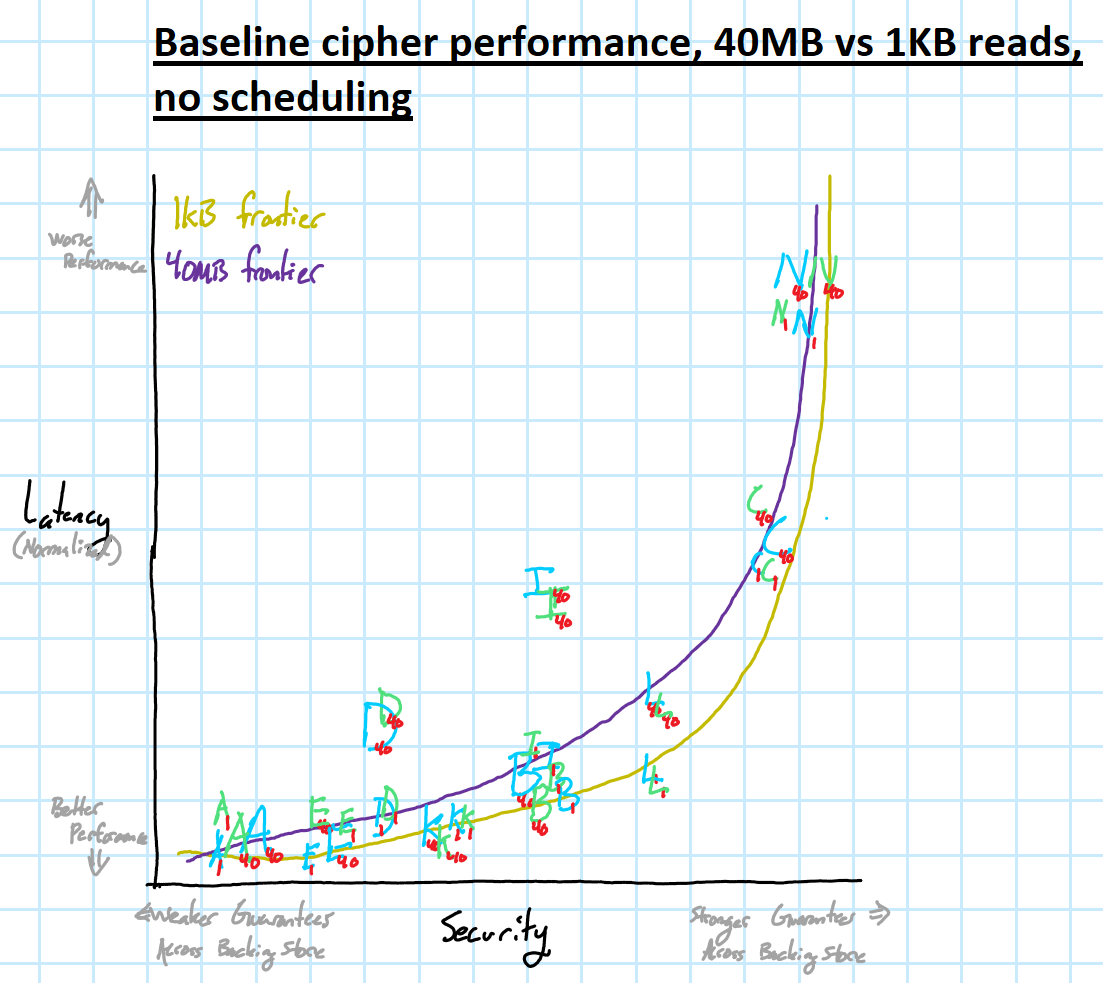
\includegraphics[width=\linewidth]{drawn/2.png}
   \caption{\TODO{Caption goes here}\TODO{Necessary? Or can we simply explain the curves are congruent with the original?}}\label{fig:40mb-vs-1kb-read}
\end{figure}

\begin{figure}[ht]
 \centering
  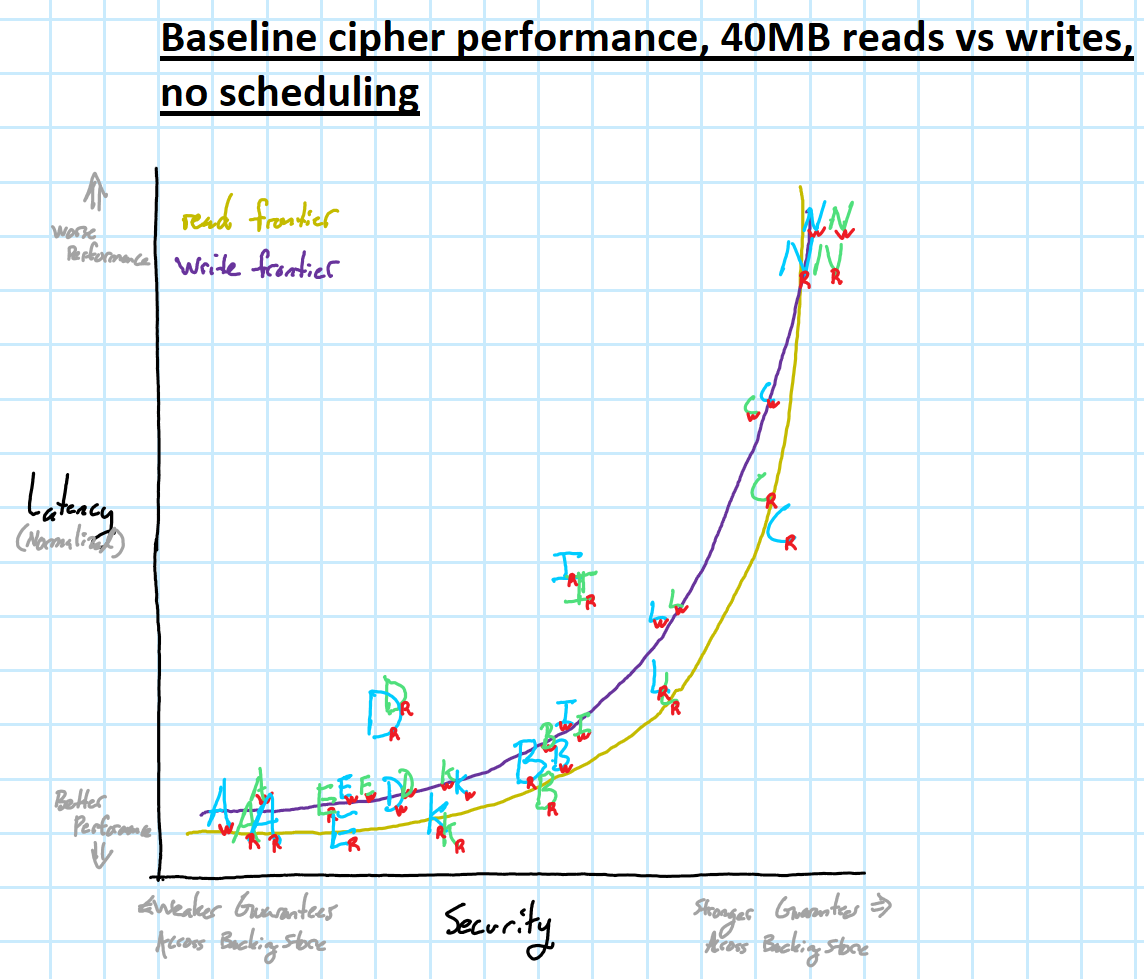
\includegraphics[width=\linewidth]{drawn/3.png}
   \caption{\TODO{Caption goes here}\TODO{Necessary? Or can we simply explain the curves are congruent with the original?}}\label{fig:40mb-read-vs-write}
\end{figure}

\begin{figure}[ht]
 \centering
  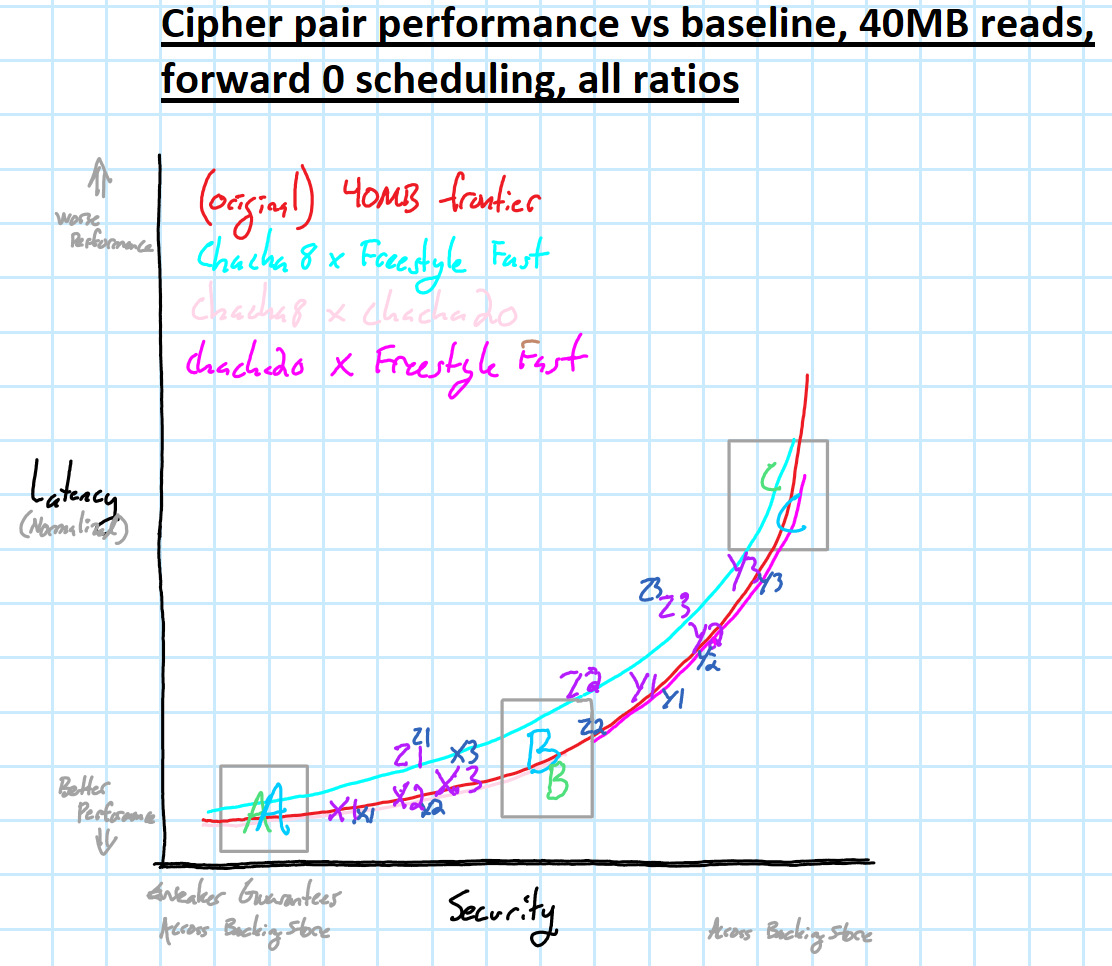
\includegraphics[width=\linewidth]{drawn/4.png}
   \caption{\TODO{Caption goes here}}\label{fig:navigating-the-space}
\end{figure}

\figref{navigating-the-space} shows the performance of \SYSTEM{} using the
0-forward switching strategy. We focus on three ciphers: ChaCha8, ChaCha20, and
Freestyle in its "fast" configuration. \TODO{Should there be a "ciphers" section
somewhere that describes all the various ciphers and cipher configurations?
Would that go in the design section?}

\begin{figure}[ht]
 \centering
  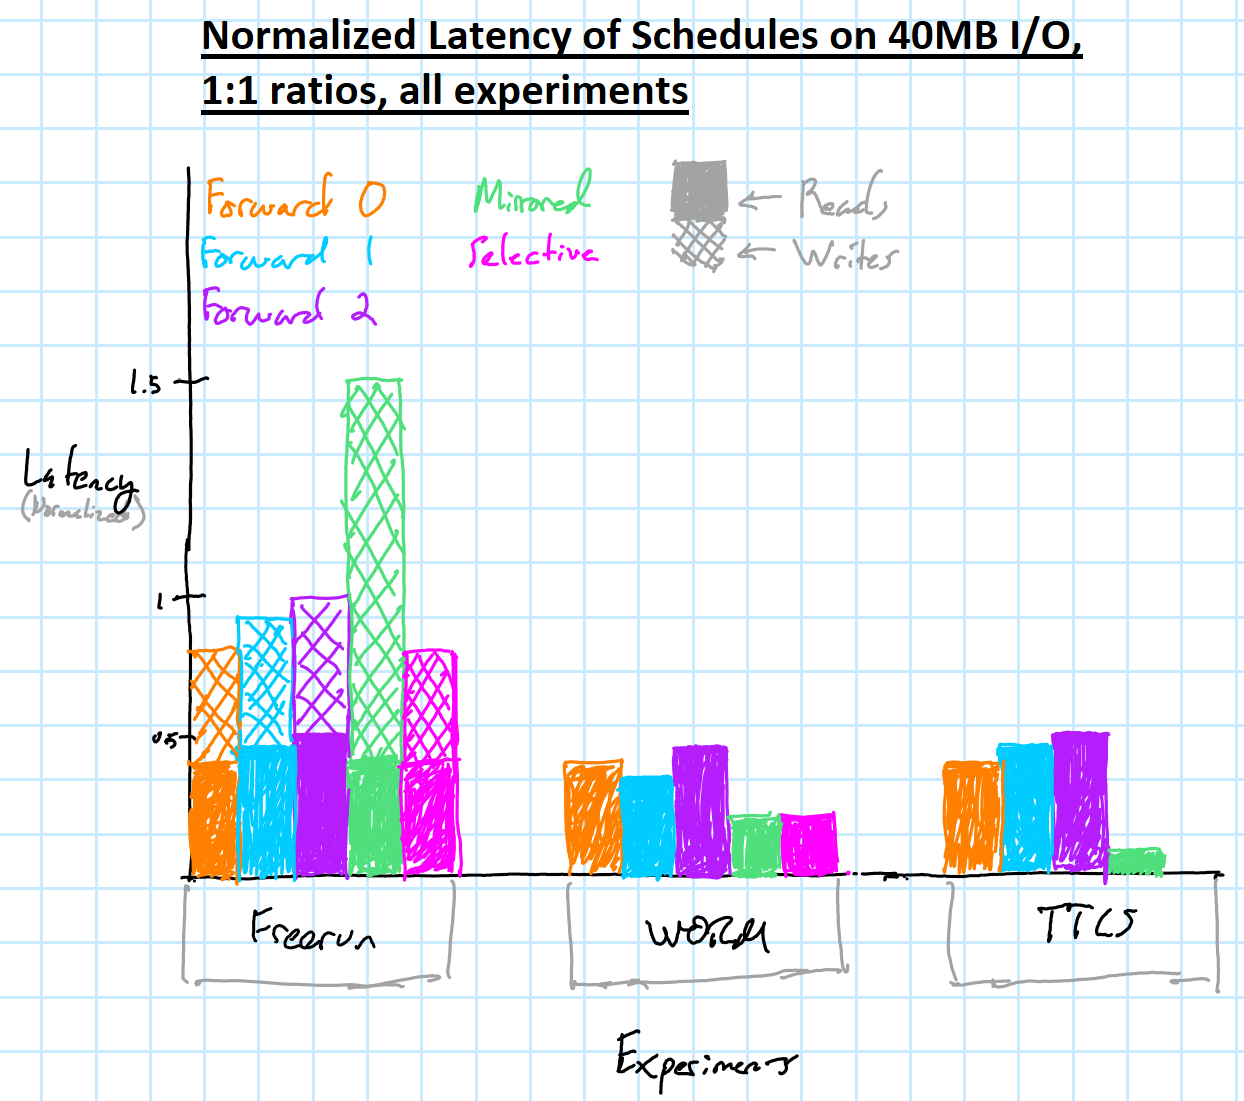
\includegraphics[width=\linewidth]{drawn/9.png}
   \caption{\TODO{Caption goes here}}\label{fig:strategy-vs-strategy}
\end{figure}

\TODO{Evaluate switching strategies against themselves. Different workloads,
different size, etc. Show that overhead is low. Show that performance is
maintained.}

\TODO{Paper up until this point makes assertions about static, offline, not
flexible. Evaluation shows flexibility.}

\TODO{Show the graph that demonstrates that we have a method to navigate this
space.}

\TODO{What assertions were made? Show results that demonstrate this.}

\TODO{This stuff works. Next section, show usefulness in practical
circumstances.}

\TODO{A point somewhere about when to use different strategies. List of concerns
that determine when to switch to what and why.}

\section{SwitchCrypt Case Studies}\label{sec:usecases}

\TODO{You need some sort of overview paragraph that tells people what is to come
in this section and why they should care about it. For example, you want to say
something about these case studies cover a wide range of situations including...
They also demonstrate uses of both temporal and spatial switching... Basically,
make the argument that these case studies provide good coverage of all the
things that you discussed earlier in the paper.}

\subsection{Balancing Security Goals with a Constrained Energy Budget}

This usecase illustrates that, because latency and energy use are correlated
among the ciphers we examined, we can exploit that property using temporal
Forward switching to save our battery. We revisit the motivating example from
\secref{motivation}, demonstrating that the ability to re-cipher individual
nuggets allows us to complete our task while staying within our energy budget.

\TODO{We may need to say something about how/why these file sizes were chosen. We want to make it clear that they are not magic numbers and the results would hold with different sizes.}
We begin sequentially writing 10 40MB files using the Freestyle Balanced cipher
configuration. After 5 seconds, the device enters ``battery saver'' mode. We
simulate this event by 1) underclocking the cores to their lowest frequencies
and 2) using \texttt{taskset} to transition the SwitchCrypt processes to the
energy-efficient LITTLE cores. Afterwards, we complete the remaining workload
using the ChaCha8 cipher. We repeat this experiment three times.

\begin{figure}[ht] \textbf{Batter Saver Use Case: Energy-Security Tradeoff vs
   Strict Energy Budget}\par\medskip
   \centering
   {\begin{tikzpicture}[baseline]

    \pgfmathsetmacro{\xmax}{130} % set the maximum x value
    \pgfmathsetmacro{\ymax}{50} % set the maximum y value
    \pgfmathsetmacro{\ymaxbreak}{50.1} % set the y value at which overflow is drawn

    \begin{groupplot}[
        group style={
            group size=1 by 2,
            ylabels at=edge left,
            xlabels at=edge bottom,
            yticklabels at=edge left,
            xticklabels at=edge bottom,
            vertical sep=10pt,
        },
        %axis x line*=bottom,
        height=4cm,
        width=\linewidth,
        tick align=outside,
        tick pos=bottom, % make sure ticks only appear at the bottom and left axes
        tick style={ black },
        y tick label style={ /pgf/number format/fixed, /pgf/number format/precision=0 },
        grid style={ dotted, gray },
        every node near coord/.append style={font=\tiny},
        %
        % % magic to make the numbers appear above the overly long bars:
        % visualization depends on={rawy \as \rawy}, % save original y values
        % restrict y to domain*={ % now clip/restrict any y value to ymax
        %     \pgfkeysvalueof{/pgfplots/ymin}:\ymaxbreak
        % },
        % after end axis/.code={ % draw squiggly line indicating break
        %     \draw [semithick, white, decoration={snake,amplitude=0.1mm,segment length=0.75mm,post length=0.375mm}, decorate] (rel axis cs:0,1.01) -- (rel axis cs:1,1.01);
        % },
        % nodes near coords={\color{.!75!black}\pgfmathprintnumber\rawy}, % print the original y values (darkened in case they're too light)...
        % nodes near coords greater equal only=\ymax, % ... but ONLY if they're >= ymax
        clip=true, % allow clip to protrude beyond ymax if false
        % % Custom stuff to edit per template
        %
        xlabel={Time (s)},
        xlabel near ticks,
        xlabel shift={-4mm},
        xmin=0, xmax=\xmax,
        xtick={ 0, \xmax },
        enlargelimits=false, % add some breathing room along the x axis's sides
        % %major x tick style=transparent,
        %
        ylabel near ticks,
        ylabel shift={-5mm},
        ymajorgrids=true,
        %yticklabels={ 0, 0.5, 1.5, 2 },
        % extra y ticks={1},
        % extra y tick style={grid=major, grid style={dashed, black}},
        % extra y tick label={\empty},
        %bar width=4.5pt, % change size of bars
        %
        legend cell align=center,
        legend style={ column sep=1ex },
        legend entries={
            {\scriptsize Freestyle Balanced},
            {\scriptsize Freestyle Balanced + ChaCha8},
            {\scriptsize ChaCha8},
        },
        legend style={
            draw=none,
            legend columns=2,
            at={(0.5, 1.02)},
            anchor=south,
        },
    ]
        \nextgroupplot[ylabel={Energy Used (j)}, ymin=0, ymax=\ymax, ytick={ 0, \ymax }]
            \addplot [thick] table [
                x=time,
                y=energy,
                discard if symbol not={cipher}{fb},
                discard if symbol not={iop}{w},
                col sep=space,
                mark=none
            ] {charts/usecase-battery.dat};
            \addplot [thick, dashdotted] table [
                x=time,
                y=energy,
                discard if symbol not={cipher}{fb+c8},
                discard if symbol not={iop}{w},
                col sep=space,
                mark=none
            ] {charts/usecase-battery.dat};
            \addplot [thick, densely dashed] table [
                x=time,
                y=energy,
                discard if symbol not={cipher}{c8},
                discard if symbol not={iop}{w},
                col sep=space,
                mark=none
            ] {charts/usecase-battery.dat};
            \coordinate (c1) at (35, 24);
            \coordinate (c2) at (89, 45);
            \coordinate (c3) at (0, 45);
            \draw [dotted] (0, 34) -- (130, 34) node [above of=c1] {\tiny (energy max)};
            \draw [dotted] (120, 0) -- (120, 50) node [right of=c2] {\tiny (battery dies)};
            \draw [dotted] (5, 0) -- (5, 50) node [right of=c3] {\tiny (battery critical)};
        \nextgroupplot[legend to name={throwaway7}, ylabel={Security Score}, ymin=0, ymax=3, ytick={ 0, 3 }]
            \addplot [thick] table [
                x=time,
                y=score,
                discard if symbol not={cipher}{fb},
                discard if symbol not={iop}{w},
                col sep=space
            ] {charts/usecase-battery.dat};
            \addplot [thick, dashdotted] table [
                x=time,
                y=score,
                discard if symbol not={cipher}{fb+c8},
                discard if symbol not={iop}{w},
                col sep=space
            ] {charts/usecase-battery.dat};
            \addplot [thick, densely dashed] table [
                x=time,
                y=score,
                discard if symbol not={cipher}{c8},
                discard if symbol not={iop}{w},
                col sep=space
            ] {charts/usecase-battery.dat};
            \coordinate (c4) at (35, 1.32);
            \draw [dotted] (120, 0) -- (120, 3);
            \draw [dotted] (5, 0) -- (5, 3);
            \draw [dotted] (0, 0.55) -- (130, 0.55) node [below of=c4] {\tiny (security floor)};
    \end{groupplot}%
\end{tikzpicture}%
} \caption{Median sequential write total
   energy use with respect to time and security score with respect to time.}
  \label{fig:usecase-battery}
\end{figure}

In \figref{usecase-battery}, we see time versus energy used and average security
score of the backing store. At 0 seconds, we begin writing. At 5 seconds, the
``battery critical'' event occurs, causing the system to be underclocked. At 120
seconds, the system will die. If we blow past our energy ceiling, the system
will die.

Our goal is to finish downloading the file before the device dies. We have three
cipher configuration choices. 1) Favor security and use Freestyle Balanced
exclusively. Our results show that the device will die before completing the
download. 2) Favor low energy use with ChaCha8 exclusively. Our results show
that the device will finish writing early, but we fall below our minimum
security score constraint. Finally, we have 3) favor security and use Freestyle
Balanced except when the system enters a low power state, after which the
storage layer switches to favoring optimal energy use using ChaCha20 via the
Forward switching strategy. Our results show that, while the system uses
slightly more power in the short term, we stay within our energy budget and
finish before the devices dies. Further, when we get our device to a charger,
SwitchCrypt can converge nuggets back to Freestyle Balanced.

On average, using Forward cipher switching results in a \TODO{XXX} total energy
use reduction.

\subsection{Variable Security Regions}

This usecase illustrates utility of spatial Selective switching to achieve a
performance win over prior work, where the entire drive is encrypted with a
single cipher. We demonstrate \emph{Variable Security Regions} (VSR), where we
can choose to encrypt select files or portions of files with different keys and
ciphers below the filesystem level. 

The goal is that if only a small percentage
of the data needs the strongest encryption, then only a small percentage of the
data should have that associated overhead.  Using prior techniques, either all 
the data would be stored with high overhead, the critical data would be stored 
without sufficient security, or the data would have to be split among separate 
files and stored across partitioned stores.

Communicating classified materials, corporate secrets, etc. require the highest
level of discretion when handled, yet sensitive information like this can
appears within a (much) larger amount of data that we value less. In this
scenario, a user wants to indicate one or more regions of a file are more
sensitive than the others. For example, perhaps banking transaction information
is littered throughout a document; perhaps passwords and other sensitive
information exists within several much larger files.

We begin by writing 10 5MB and 4KB files to unique SwitchCrypt instances using
ChaCha8 and again on instances using Freestyle Balanced. We repeat this on a
SwitchCrypt instance using Selective switching with a 3:1 ratio of ChaCha8
nugget I/O operations versus Freestyle Balanced operations. We repeat this
experiment three times.

\begin{figure}[ht] \textbf{VSR Use Case: ChaCha8 vs Freestyle Secure Sequential
4KB, 5MB Performance}\par\medskip
   \centering
   {\begin{tikzpicture}[baseline]

    \pgfmathsetmacro{\ymax}{20} % set the maximum y value
    \pgfmathsetmacro{\ymaxbreak}{20.1} % set the y value at which overflow is drawn

    \begin{axis}[
        %axis x line*=bottom,
        height=4cm,
        width=\linewidth,
        tick align=outside,
        tick pos=bottom, % make sure ticks only appear at the bottom and left axes
        tick style={ black },
        y tick label style={ /pgf/number format/fixed, /pgf/number format/precision=0 },
        grid style={ dotted, gray },
        every node near coord/.append style={font=\tiny},
        %
        % magic to make the numbers appear above the overly long bars:
        visualization depends on={rawy \as \rawy}, % save original y values
        restrict y to domain*={ % now clip/restrict any y value to ymax
            \pgfkeysvalueof{/pgfplots/ymin}:\ymaxbreak
        },
        after end axis/.code={ % draw squiggly line indicating break
            \draw [semithick, white, decoration={snake,amplitude=0.1mm,segment length=0.75mm,post length=0.375mm}, decorate] (rel axis cs:0,1.01) -- (rel axis cs:1,1.01);
        },
        nodes near coords={\color{.!75!black}\pgfmathprintnumber\rawy}, % print the original y values (darkened in case they're too light)...
        nodes near coords greater equal only=\ymax, % ... but ONLY if they're >= ymax
        clip=false, % allow clip to protrude beyond ymax
        % Custom stuff to edit per template
        %
        xlabel={\footnotesize Cipher Configuration},
        xlabel near ticks,
        xmin=C8, xmax=FS,
        xtick=data,
        symbolic x coords={C8,C8+FS,FS},
        enlarge x limits=0.2, % add some breathing room along the x axis's sides
        %major x tick style=transparent,
        %
        ylabel={\footnotesize Latency (s)},
        ylabel near ticks,
        ylabel shift={-1mm},
        ymajorgrids=true,
        ymin=0, ymax=\ymax,
        ybar, % value will shift bars
        ytick={ 0, 5, ..., \ymax },
        %yticklabels={ 0, 0.5, 1.5, 2 },
        % extra y ticks={1},
        % extra y tick style={grid=major, grid style={dashed, black}},
        % extra y tick label={\empty},
        %bar width=4.5pt, % change size of bars
        %
        legend cell align=center,
        legend style={ column sep=1ex },
        legend entries={
            {\scriptsize 4K/reads},
            {\scriptsize 4K/writes},
            {\scriptsize 5M/reads},
            {\scriptsize 5M/writes},
        },
        legend style={
            draw=none,
            legend columns=2,
            at={(0.5,1.02)},
            anchor=south,
        },
    ]
        \addplot[fill=orangeDark, every node near coord/.append style={color=orangeDark}]
        table[x=conf, y=latr-4k, col sep=space] {charts/usecase-vsr-tradeoff.dat};
        \addplot[fill=orangeDark, postaction={pattern=north east lines}, every node near coord/.append style={color=purpleDark}]
        table[x=conf, y=latw-4k, col sep=space] {charts/usecase-vsr-tradeoff.dat};
        \addplot[fill=purpleDark, every node near coord/.append style={color=orangeDark}]
        table[x=conf, y=latr-5m, col sep=space] {charts/usecase-vsr-tradeoff.dat};
        \addplot[fill=purpleDark, postaction={pattern=north east lines}, every node near coord/.append style={color=purpleDark}]
        table[x=conf, y=latw-5m, col sep=space] {charts/usecase-vsr-tradeoff.dat};
    \end{axis}%
\end{tikzpicture}%
} \caption{Median sequential read and
   write performance comparison of 5MB I/O with 3-to-1 ratio of ChaCha8 nuggets
   to Freestyle Secure nuggets, respectively.}
  \label{fig:usecase-vsr-bar}
\end{figure}

In \figref{usecase-vsr-bar}, we see the sequential read and write performance of
4K and 5M workloads when nuggets are encrypted exclusively with ChaCha8 or
Freestyle Balanced. Between them, we see SwitchCrypt Selective switching 3:1
ratio I/O results.

Our goal is to use VSRs to keep our sensitive data secure while keeping the
performance and energy use benefits of using a fast cipher for the majority of
I/O operations. On average, using SwitchCrypt Selective switching versus prior
work results in a \TODO{XXX} reduction in latency.

\subsection{Responding to End-of-Life Slowdown in Solid State Drives}

This usecase illustrates using temporal Forward switching to offset the
debilitating decline in performance when SSDs reach end-of-life
(EoL)~\cite{SSDEOL1, SSDEOL2, SSDEOL3}. We demonstrate the utility of such a
system to dynamically stay within a strict latency budget while meeting minimum
security requirements, which is not possible using prior work.

Due to garbage collection and wear-leveling requirements of SSDs, as free space
becomes constrained, I/O performance drops precipitously~\cite{SSDEOL1, SSDEOL2,
SSDEOL3}. With prior work, our strict latency ceiling is violated. However, if
SwitchCrypt is made aware when the backing store is in such a state, we can
offset some of the performance loss by switching the ciphers of high traffic
nuggets to the fastest cipher available using Forward switching.

We begin by writing 10 40MB files to SwitchCrypt per each cipher as a baseline.
We then introduce a delay into SwitchCrypt I/O of $20ms$ and repeat the
experiment three times.

\begin{figure}[ht] \textbf{SSD EoL Use Case: Latency-Security Tradeoff vs
   Goals}\par\medskip
   {\begin{tikzpicture}[baseline]

    \pgfmathsetmacro{\ymax}{1.1} % set the maximum y value
    \pgfmathsetmacro{\ymaxbreak}{1.2} % set the y value at which overflow is drawn

    \begin{groupplot}[
        group style={
            group size=2 by 2,
            xlabels at=edge bottom,
            ylabels at=edge left,
            xticklabels at=edge bottom,
            yticklabels at=edge left,
            vertical sep=25pt,
            horizontal sep=15pt,
        },
        %axis x line*=bottom,
        scatter,
        point meta=explicit,
        scatter/classes={
            1={},
            2={dashed},
            3={mark=triangle*,red,mark size=2.5pt},
            4={mark=triangle*,orange,mark size=3pt},
            5={mark=square*,blue,mark size=2pt}
        },
        height=6cm,
        width=\textwidth/2,
        tick align=outside,
        %tick pos=bottom, % make sure ticks only appear at the bottom and left axes
        title style={yshift=-1.5ex},
        tick style={ black },
        y tick label style={ /pgf/number format/fixed, /pgf/number format/precision=0 },
        grid style={ dotted, gray },
        %every node near coord/.append style={font=\tiny},
        %
        % magic to make the numbers appear above the overly long bars:
        % visualization depends on={rawy \as \rawy}, % save original y values
        % restrict y to domain*={ % now clip/restrict any y value to ymax
        %     \pgfkeysvalueof{/pgfplots/ymin}:\ymaxbreak
        % },
        % after end axis/.code={ % draw squiggly line indicating break
        %     \draw [semithick, white, decoration={snake,amplitude=0.1mm,segment length=0.75mm,post length=0.375mm}, decorate] (rel axis cs:0,1.01) -- (rel axis cs:1,1.01);
        % },
        % nodes near coords={\color{.!75!black}\pgfmathprintnumber\rawy}, % print the original y values (darkened in case they're too light)...
        % nodes near coords greater equal only=\ymax, % ... but ONLY if they're >= ymax
        % clip=false, % allow clip to protrude beyond ymax
        % Custom stuff to edit per template
        %
        xlabel={\footnotesize Security Score},
        xlabel near ticks,
        %xlabel shift={-1.5mm},
        xmin=0, xmax=4,
        xtick={ 0, 1, 2, 3, 4 },
        xticklabels={ 0,,, 3, \empty },
        major x tick style=transparent,
        %enlarge x limits=0.2, % add some breathing room along the x axis's sides
        %
        ylabel={\footnotesize Latency (normalized)},
        ylabel near ticks,
        ylabel shift={-1.5mm},
        ymajorgrids=true,
        ymin=0, ymax=\ymax,
        ytick={ 0, 1, \ymax },
        yticklabels={ 0, 1, \empty },
        %yticklabels={ 0, 0.5, 1.5, 2 },
        % extra y ticks={1},
        % extra y tick style={grid=major, grid style={dashed, black}},
        % extra y tick label={\empty},
        %bar width=4.5pt, % change size of bars
        %
        legend cell align=center,
        legend style={ column sep=1ex },
        legend entries={%
            {\scriptsize Normal},
            {\scriptsize Delayed},
            {\scriptsize Choice Config (Normal)},
            {\scriptsize Bad Config (Delayed)},
            {\scriptsize Choice Config (Delayed)}
        },
        legend style={
            draw=none,
            legend columns=3,
            at={(1.0,1.2)},
            anchor=south,
        },
    ]
        \nextgroupplot[title={Sequential Reads}]
            \addplot [thick] table [
                meta=label,
                x=score,
                y=latency,
                discard if symbol not={iop}{r},
                discard if symbol not={delayed}{no},
                discard if symbol not={order}{seq},
                col sep=space,
            ] {charts/usecase-eol-tradeoff.dat};
            \addplot [thick, dashed] table [
                meta=label,
                x=score,
                y=latency,
                discard if symbol not={iop}{r},
                discard if symbol not={delayed}{yes},
                discard if symbol not={order}{seq},
                col sep=space
            ] {charts/usecase-eol-tradeoff.dat};
            \coordinate (c1) at (205, 85);
            \coordinate (c2) at (60, 9);
            \draw [dotted] (190, 0) -- (190, 110) node [left of=c1] {\tiny (security floor)};
            \draw [dotted] (0, 30) -- (400, 30) node [above of=c2] {\tiny (latency ceiling)};
        \nextgroupplot[legend to name={throwaway9}, title={Random Reads}]
            \addplot [thick] table [
                meta=label,
                x=score,
                y=latency,
                discard if symbol not={iop}{r},
                discard if symbol not={delayed}{no},
                discard if symbol not={order}{rnd},
                col sep=space
            ] {charts/usecase-eol-tradeoff.dat};
            \addplot [thick, dashed] table [
                meta=label,
                x=score,
                y=latency,
                discard if symbol not={iop}{r},
                discard if symbol not={delayed}{yes},
                discard if symbol not={order}{rnd},
                col sep=space
            ] {charts/usecase-eol-tradeoff.dat};
            \coordinate (c3) at (205, 85);
            \coordinate (c4) at (60, 9);
            \draw [dotted] (190, 0) -- (190, 110) node [left of=c3] {\tiny (security floor)};
            \draw [dotted] (0, 30) -- (400, 30) node [above of=c4] {\tiny (latency ceiling)};
        \nextgroupplot[legend to name={throwaway10}, title={Sequential Writes}]
            \addplot [thick] table [
                meta=label,
                x=score,
                y=latency,
                discard if symbol not={iop}{w},
                discard if symbol not={delayed}{no},
                discard if symbol not={order}{seq},
                col sep=space
            ] {charts/usecase-eol-tradeoff.dat};
            \addplot [thick, dashed] table [
                meta=label,
                x=score,
                y=latency,
                discard if symbol not={iop}{w},
                discard if symbol not={delayed}{yes},
                discard if symbol not={order}{seq},
                col sep=space
            ] {charts/usecase-eol-tradeoff.dat};
            \coordinate (c5) at (205, 85);
            \coordinate (c6) at (60, 9);
            \draw [dotted] (190, 0) -- (190, 110) node [left of=c5] {\tiny (security floor)};
            \draw [dotted] (0, 30) -- (400, 30) node [above of=c6] {\tiny (latency ceiling)};
        \nextgroupplot[legend to name={throwaway11}, title={Random Writes}]
            \addplot [thick] table [
                meta=label,
                x=score,
                y=latency,
                discard if symbol not={iop}{w},
                discard if symbol not={delayed}{no},
                discard if symbol not={order}{rnd},
                col sep=space
            ] {charts/usecase-eol-tradeoff.dat};
            \addplot [thick, dashed] table [
                meta=label,
                x=score,
                y=latency,
                discard if symbol not={iop}{w},
                discard if symbol not={delayed}{yes},
                discard if symbol not={order}{rnd},
                col sep=space
            ] {charts/usecase-eol-tradeoff.dat};
            \coordinate (c7) at (205, 85);
            \coordinate (c8) at (60, 9);
            \draw [dotted] (190, 0) -- (190, 110) node [left of=c7] {\tiny (security floor)};
            \draw [dotted] (0, 30) -- (400, 30) node [above of=c8] {\tiny (latency ceiling)};
    \end{groupplot}%
\end{tikzpicture}%
} \caption{Median sequential and
   random 40MB read and write performance comparison: baseline versus simulated
   faulty block device.}
  \label{fig:usecase-eol-tradeoff}
\end{figure}

In \figref{usecase-eol-tradeoff}, we see the sequential and random read and
write performance of a 40MB workload when nuggets are encrypted exclusively with
our choice ciphers. While the latency ceiling and security floor have not
changed, we see increased latency in the delayed workloads.

Our goal is to remain under the latency ceiling while remaining above the
security floor. Thanks to Forward switching, accesses to highly trafficked areas
of the drive can remain performant even during EoL.

\subsection{Custody Panic: Securing Device Data Under Duress}

This usecase illustrates the utility of spatial Mirrored switching to take
advantage of more energy-efficient high-performance ciphers while retaining the
ability to quickly converge the entire backing store to a single high-security
cipher leveraging SSD Instant Secure Erase (ISE).

Nation-state and other ``adversaries'' have extensive compute resources,
knowledge of side-channels, and access to technology like q-bit computers. \TODO{Do you mean quantum?}
Suppose a scientist were attempting to re-enter her country through a border
entry point when she is stopped. Further suppose her laptop containing sensitive
priceless research data is confiscated from her custody. Being a security
researcher, she has a chance to trigger a remote wipe, where the laptop uses
Instant Secure Erase to reset its internal storage, permanently destroying all
her data. While she certainly doesn't want her data falling into the wrong
hands, she cannot afford to lose that data either. In such a scenario, it would
be useful if, instead of destroying the data, the storage layer could switch
itself to a more secure state as quickly as possible.

\begin{figure}[ht] \textbf{Custody Panic Use Case: Security Goals vs Time
Constraint}\par\medskip
   \centering
   {\begin{tikzpicture}[baseline]
    \begin{groupplot}[
        % 6 seconds (0.3) + 3 seconds (0.15) + 11 seconds (0.55) = 1.0
        no marks,
        group style={
            group size=1 by 2,
            xlabels at=edge bottom,
            ylabels at=edge left,
            %xticklabels at=edge bottom,
            yticklabels at=edge left,
            vertical sep=35pt,
            horizontal sep=15pt,
        },
        %axis x line*=bottom,
        height=4cm,
        width=\linewidth/1.25,
        tick align=outside,
        tick pos=bottom, % make sure ticks only appear at the bottom and left axes
        title style={yshift=-1.5ex},
        tick style={ black },
        y tick label style={ /pgf/number format/fixed, /pgf/number format/precision=0 },
        grid style={ dotted, gray },
        point meta=explicit symbolic,
        scatter/classes={
            c8={mark=square*},
            c20={mark=triangle*, red},
            ff={mark=diamond*},
            fb={mark=pentagon*},
            fs={mark=otimes, red}
        },
        %every node near coord/.append style={font=\tiny},
        %
        % magic to make the numbers appear above the overly long bars:
        % visualization depends on={rawy \as \rawy}, % save original y values
        % restrict y to domain*={ % now clip/restrict any y value to ymax
        %     \pgfkeysvalueof{/pgfplots/ymin}:\ymaxbreak
        % },
        % after end axis/.code={ % draw squiggly line indicating break
        %     \draw [semithick, white, decoration={snake,amplitude=0.1mm,segment length=0.75mm,post length=0.375mm}, decorate] (rel axis cs:0,1.01) -- (rel axis cs:1,1.01);
        % },
        % nodes near coords={\color{.!75!black}\pgfmathprintnumber\rawy}, % print the original y values (darkened in case they are too light)...
        % nodes near coords greater equal only=\ymax, % ... but ONLY if they are >= ymax
        % clip=false, % allow clip to protrude beyond ymax
        % Custom stuff to edit per template
        %
        xlabel near ticks,
        xlabel shift={-0.5mm},
        xmin=0, xmax=1,
        %enlarge x limits=0.2, % add some breathing room along the x axis's sides
        %
        ylabel near ticks,
        %ylabel shift={-1.5mm},
        ymajorgrids=false,
        ymin=0, ymax=4,
        ytick={ 0, 1, 1.5, 2, 3, 4 },
        yticklabels={ 0,,1.5,, 3, \empty },
        major y tick style=transparent,
        %yticklabels={ 0, 0.5, 1.5, 2 },
        % extra y ticks={1},
        % extra y tick style={grid=major, grid style={dashed, black}},
        % extra y tick label={\empty},
        %bar width=4.5pt, % change size of bars
        %
        legend cell align=center,
        legend style={ column sep=1ex },
        legend entries={%
            {\scriptsize Mirrored Scores (Without SwitchCrypt)},
            {\scriptsize Desired Minimum Score},
            {\scriptsize Actual Minimum Score (SwitchCrypt)}
        },
        legend style={
            draw=none,
            legend columns=2,
            at={(0.5,1.2)},
            anchor=south,
        },
    ]
        \nextgroupplot[
            xlabel={\footnotesize Time (s)},
            ylabel={\footnotesize Security Score},
            xtick={ 0, 0.3, 0.45, 1 },
            xticklabels={ 0, 6, 9, \ldots },
        ]
            \addplot [thick, red] table [
                x=time,
                y=score,
                discard if number not={line}{1},
                col sep=space
            ] {charts/usecase-custody.dat};
            \addplot [thick, red, forget plot] table [
                x=time,
                y=score,
                discard if number not={line}{3},
                col sep=space
                ] {charts/usecase-custody.dat};
            \addplot [thick, densely dotted, blue] table [
                x=time,
                y=score,
                discard if number not={line}{2},
                col sep=space
                ] {charts/usecase-custody.dat};
            \addplot [thick, dashed, blue] table [
                x=time,
                y=score,
                discard if number not={line}{4},
                col sep=space,
                ] {charts/usecase-custody.dat};
            \coordinate (c1) at (0.375, 3.5);
            \coordinate (c2) at (0.415, 3.5);
            \draw [dotted, black] (0.2945, 0) -- (0.2945, 4) node [left of=c1] {\tiny (panic; ISE)};
            \draw [dotted, black] (0.455, 0) -- (0.455, 4) node [right of=c2] {\tiny (ISE completes)};
        \nextgroupplot[
            scatter,
            legend to name={throwaway8},
            xlabel={\footnotesize Latency (normalized)},
            ylabel={\footnotesize Security Score},
            xtick={ 0, 1 },
            xticklabels={ 0, 1 },
        ]
            \addplot [thick] table [
                meta=cipher,
                x=latency,
                y=score,
                discard if symbol not={iop}{40m-r},
                discard if symbol not={order}{seq},
                col sep=space
            ] {charts/tradeoff-baseline.dat};
            \coordinate (c3) at (0.27, 1.75);
            \coordinate (c4) at (0.755, 0.5);
            \draw [dotted] (0.035, 0) -- (0.035, 4) node [above of=c3] {\tiny (pre-panic latency ceiling)};
            \draw [dotted] (0.999, 0) -- (0.999, 4) node [above of=c4] {\tiny (post-panic latency ceiling)};
    \end{groupplot}%
\end{tikzpicture}%
} \caption{Actual security score vs
   security goal with respect to the time and ISE.}
  \label{fig:usecase-custody}
\end{figure}

In \figref{usecase-eol-tradeoff}, we see the system begins at 0 seconds, where
all data is mirrored across the backing store (perhaps consisting of multiple
physical drives). Both the desired and minimum security score of the drive is
1.5, a balance between performance and security. At 6 seconds, custody panic is
triggered---the desired minimum security score goes to 3, the highest possible---at which point the
system executes ISE and completely erases the drive containing the minimally
scored data. ISE is known to be much faster than TRIM and completes in as little
as 3 seconds~\cite{SeaGate,Samsung,ThatOtherOEM}. Once complete, the most secure
form of the data is all that remains. The backing store has been ``locked
down.''

Our goal is to lock down the backing store, slowing down any attacker as
much as possible such that, even if they copy and permanently store her data
off-site for later attempts at decryption with more advanced compute resources
and new technologies, our researcher's data is some degree more likely to remain
irrecoverable. We show that, given a device that supports SSD ISE, SwitchCrypt,
and the Mirrored strategy, we can quickly and practically converge the backing
store to this locked down state. With prior work, data is either too weakly
encrypted or the device becomes too slow for daily use (latency ceiling). In
exchange, we trade off half of our drive's writeable space.

\TODO{Again, need some summary of what we just saw in this section.  What are the lessons learned from these four case studies?  How do they relate to the other points in the paper?}

\section{Related Work} \label{sec:related}

\TODO{A paragraph on FDE prior work; including StrongBox?}

\TODO{Include collection of papers that trade energy/perf vs securty; we're not
crazy!}

\TODO{Include LastPass work from much earlier}

\TODO{We should cite Google too. Their Adiantum project is using a reduced round
version of ChaCha!}

\section{Conclusion} \label{sec:conclusion}

\TODO{That's all, folks!}

%% Acknowledgments
\PUNT{\begin{acks}
  We would like to thank the anonymous reviewers for their insightful
  feedback and comments. This material is based upon work supported by
  the \grantsponsor{GS100000001}{\mbox{National} \mbox{Science}
    \mbox{Foundation}}{http://dx.doi.org/10.13039/100000001} under
  Grant No.~\grantnum{GS100000001}{CNS-1526304}. Any opinions,
  findings, and conclusions or recommendations expressed in this
  material are those of the author and do not necessarily reflect the
  views of the \mbox{National} \mbox{Science} \mbox{Foundation}.
\end{acks}}


% Uncomment to show all citable references:
% \cite{*}

%% Start a new page for your references:
\clearpage

%% Test printing all refs:
%\nocite{*}

%% If using natbib:
\bibliographystyle{ACM-Reference-Format}
%\balance % it doesn't seem to work with this outdated natbib thing
\bibliography{refs}

%% If using biblatex:
%\bibliographystyle{ACM-Reference-Format}
%\balance
%\printbibliography

\end{document}
